\documentclass[11pt]{article} %This sets the font size and the document class of your report. In this case we use 'article' as that is ideal for shorter reports.
\usepackage{amssymb}
\usepackage{amsmath}
\usepackage{subcaption}
% LaTeX can be enhanced by the use of packages. These packages can do many things, a few of the most common and useful are used here. They are declared before the document proper, in what is known as the 'preamble'. Packages need to be installed when a .tex file compiles into a .pdf, but should do so automatically.
\usepackage[top=1.5cm, bottom=1.5cm, left=1.75cm, right=1.75cm]{geometry} %This sets the margins of the report.

\usepackage{graphicx} % A package allowing insertion of images into the text.
\usepackage{caption}

% Choose your citations style by commenting out one of the following groups. If you decide to change style, you should also delete the .bbl file that you will find in the same folder as your .tex and .pdf files.

% IEEE style citation:
\usepackage[style=ieee]{biblatex}
\addbibresource{sem_2_report.bib}
\DeclareMathOperator{\E}{\mathbb{E}}
\DeclareMathOperator{\Var}{\mathrm{Var}}


\usepackage{enumerate}
%% Author-date style citation:
%\usepackage[round]{natbib} % A package that creates references in the author-date style, with round brackets
%\renewcommand{\cite}{\citep} % For use with natbib only: comment out for the cite package.
%\bibliographystyle{plainnat} % Author-date referencing (use in conjunction with the natbib package)
\usepackage{color} % Allows the colour of the font to be changed by using the '\color' command: This is just to support the blue comments in this template...use standard (black) text in your report.
\usepackage{float}
\usepackage{subdepth}
\usepackage{mathtools}
\usepackage{tabularx}
\usepackage{makecell}
\linespread{1} % Sets the spacing between lines of text.
\setlength{\parindent}{0cm}  % Suppresses indentation of text at the start of a paragraph
\pagenumbering{arabic} % sets the style of page numbering for the report


\begin{document} % This begins the document proper and ends the pre-amble

% The last } finishes the chunk of text opening with {\color{blue}..., so all of the above appears as blue text. A common LaTeX error is to forget to close such a chunk of text, so if the formatting goes wrong look for a missing }.

% To get rid of the blue text, select and delete everything from '{\color' to '}', inclusive, leaving \ begin{titlepage} as the first command  after \begin{document}

\begin{center} % Starts the beginning of an environment where all text is centered.

{\Huge Simulating light detection in liquid argon time projection chambers for neutrino and dark matter experiments with deep learning techniques}\\[0.5cm] % [0.5cm] sets the distance between this line and the next.
\vspace{5mm}
\textit{Enrico Zammit Lonardelli}
\\
\vspace{5mm}
\text{9910821}
\\
\vspace{5mm}
\text{School of Physics and Astronomy}
\\
\vspace{5mm}
\text{The University of Manchester}
\\
\vspace{5mm}
\text{Masters Project}
\\
\vspace{5mm}
\text{May 2020}
\\
\vspace{5mm}
This experiment was performed in collaboration with \textit{Krishan Jethwa}\\[0.3cm] % The '\\' starts a new paragraph, and will only work after a paragraph has started, unless we use '~'.

\end{center}
\vspace{60mm}
{\Large \textbf{Abstract}}
\vspace{2mm}
\\
This report details the work done as part of our Masters project in the second semester as a continuation of work done in the first semester \cite{firstsemester}.
We discuss quantitative comparisons between the prestablished Monte Carlo package known as G4DS and novel deep learning methods with an AutoRegressive Generative
Adverserial Network (ARGAN) known as GAN4DS.
Furthermore, we present the results of GAN4DS on variables of light intensity $S_1$, $S_2$
 and $f_{200}$ by implicit learning of their mutual underlying conditional probabilities.
Discriminating plots between nuclear and electron recoils of $f_{200}$ vs $S_1$ and log($S_2$/$S_1$) vs $S_1$ are also presented.

\pagebreak
\section{Introduction}
\subsection{The search for signal}
\begin{figure}[H]
\centering
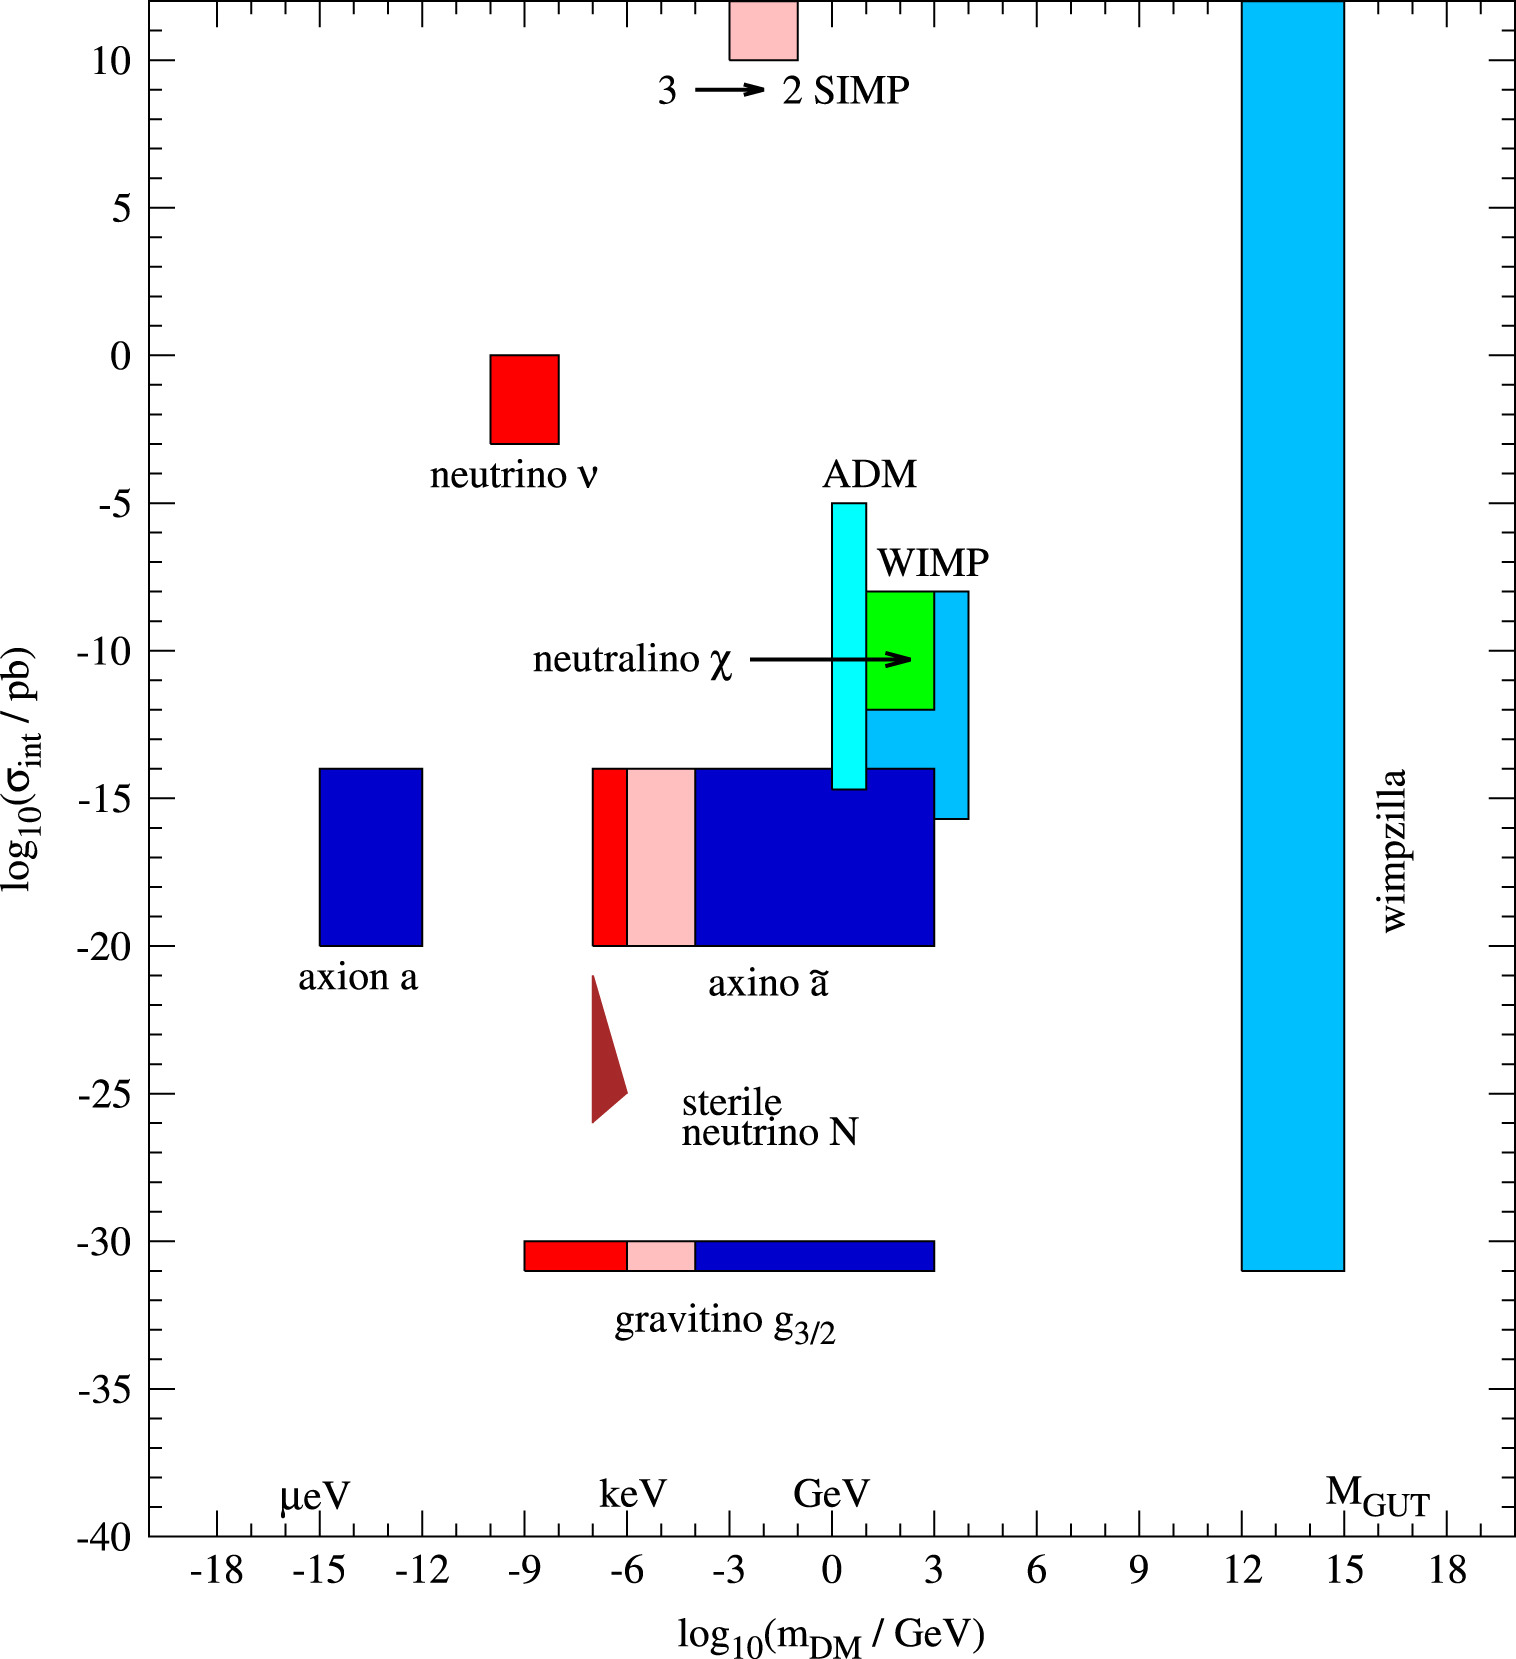
\includegraphics[scale=1]{images/mass_ranges.jpg}
\caption{\cite{BAER20151} Currently hypothesised masses for dark matter candidates from different theories.}
\label{fig:mass_ranges}
\end{figure}
\par Cosmological findings have been the driving motivation behind dark matter search for the past 90 years \cite{bertone2018history}.
The leap to a Weakly Interacting Massive Particle (WIMP) \cite{steigman1984cosmological} is not a trivial one and one must take great care in the assumptions \cite{scherrer1986relic}
it makes and why it makes them, especially in light of increasing ranges of masses being excluded by experiments running today.
The first defining feature is thus mass.
This is currently under heavy debate in the scientific community as there are supporters of a very low mass dark matter candidate (such as axions \cite{weinberg1978new} or sterile neutrinos \cite{kusenko2009sterile})
while on the other side of the spectrum most standard direct detection experiments today \cite{Agnes_2015} \cite{McKinsey_2016}  are for mass ranges running from tens to hundreds of GeV/$c^2$.
Evidence from phenomena such as gravitational lensing \cite{wittman2000detection} and the constant rotational velocities of stars in galaxies with increasing
distance to their galactic centres \cite{oort1932force} suggest a candidate of dark matter halos around these celestial objects.
\\
\par From supersymmetrical neutralinos to superheavy dark matter candidates we are looking at a range from GeV/$c^2$ to several TeV/$c^2$ and even higher in certain theories \cite{roszkowski2004particle}, see Figure \ref{fig:mass_ranges}.
What many of these theories have in common however is that they all produced these WIMP candidates as a byproduct or as required assumptions
to allow their theories to work.
This strengthens the theory that such a particle should exist and what regions of mass, energy and interaction type to look for.
These WIMPs are hypothesised to have been in thermal equilibrium with thermal plasma in the early universe.
As the universe expanded and WIMP annihilation rate was less than the Hubble expansion rate, relic density for dark matter was reached.
This brings us to the cross-sections expected for such WIMPs.
Although this varies from theory to theory, we are expecting orders of the weak interaction scale.
\\
\par This incredibly low interaction rate with regular matter makes it a challenge to detect such WIMPs.
There have been efforts at the Large Hadron Collider \cite{aad2013search} \cite{chatrchyan2012search} to detect missing energies and transverse momenta which could be
explained only through a missing new particle in the mass range of a dark matter candidate.
Although, to date, these efforts have translated into constraints of cross sections and mass the search is still active.
\\
\par Another method of search is through indirect detection \cite{gaskins2016review} by observing celestial objects which have a high mass to luminosity disparity.
These include but are not limited to galactic centres, dwarf galaxies and galaxy clusters close to ours \cite{harvey2015nongravitational}.
This method relies on closely monitoring the particle flux coming from these places waiting for self-interactions or decays into measurable standard model particles to occur.
Searches via these methods are made even harder by the fact that the only byproducts most experiments can reliably measure after accounting
for interstellar magnetic fields, other celestial objects and low background limits are neutrinos and specific gamma ray energies.
\\
\begin{figure}[H]
\centering
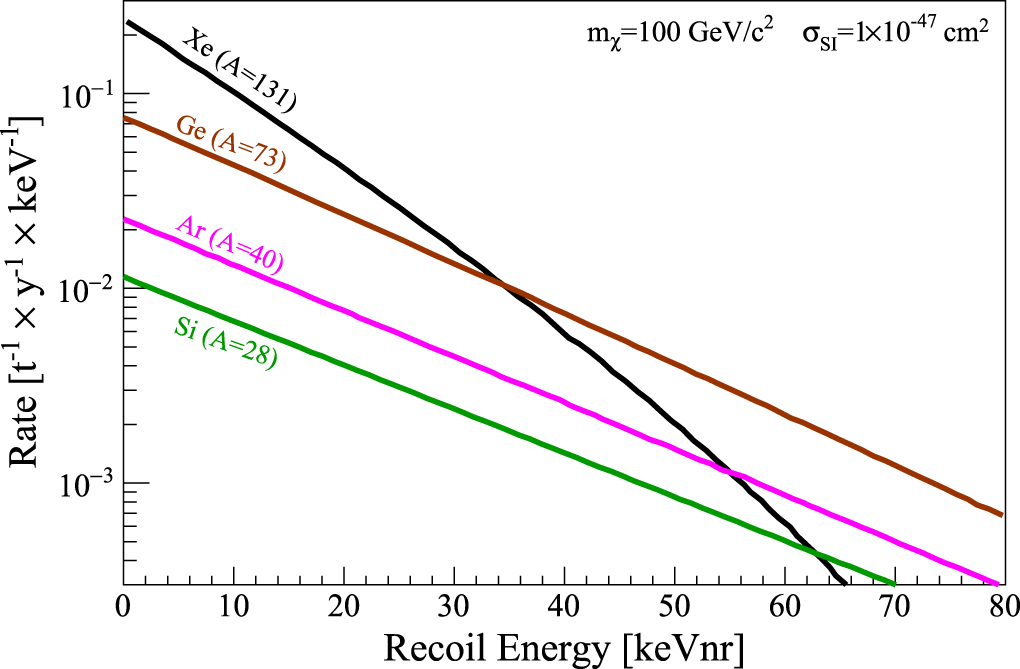
\includegraphics[scale=1]{images/recoil_spectra.jpg}
\caption{\cite{Schumann_2019} Nuclear recoil spectra for varying noble gas targets highlight the better interaction
rate at lower nuclear recoil energies for heavier targets but a lower rate for higher recoil energies.}
\label{fig:recoil_spectra}
\end{figure}
\par Finally, the last method of detection is direct detection \cite{gaitskell2004direct} and the most common one as of today's experiments.
Large detector chambers are set up, often many kilometers under the earth, essentially waiting for a WIMP
candidate to produce an elastic nuclear recoil with a noble element atom and produce measurable scintillation.
For a WIMP mass ranging between 1 GeV/$c^2$ and 1000 GeV/$c^2$ the recoil energies are in the range 1-100 keV
after which the cross-sections become way too small for modern detectors.
The choice of noble gas element to use is also non-trivial since the rate for spin-indipendent interactions increases with
nucleon number however decreases at high energies due to form factor suppression, as expressed by \cite{goodman1985detectability}
\begin{equation}
\frac{{\rm{d}}{R}}{{{\rm{d}}{E}}_{\mathrm{nr}}} = \frac{\rho_0}{m_x m_N} \int_{v_{min}}^{v_{esc}}\frac{{\rm{d}}{\sigma_{x N}}}{{{\rm{d}}{E}}_{\mathrm{nr}}}(v,E_{\mathrm{nr}}) v f(v) dv
\label{eq:dm}
\end{equation}
often approximated to \cite{lewin1996review}
\begin{equation}
\frac{{\rm{d}}{R}}{{{\rm{d}}{E}}_{\mathrm{nr}}}\propto \exp (- \frac{{E}_{\mathrm{nr}}}{{E}_{0}} \frac{4{m}_{\chi }{m}_{N}}{{({m}_{\chi }+{m}_{N})}^{2}})
\end{equation}
and shown in Figure \ref{fig:recoil_spectra} for increasing mass of the target nucleus.
Here $m_X$ is the dark matter mass, $m_N$ is the mass of the noble element, $\rho_0$ is density of dark matter in the local space,
$v_{min}$ is the dark matter velocity and depends on the annual and diurnal modulation \cite{drukier1986detecting}.
\\
\par The higher interaction rate for lower recoil energies makes it more probable to detect a WIMP candidate interaction
however these energies produce a lower intensity of scintillation which results in larger errors
(from sources such as photomultiplier calibration, photon efficiency, dark currents) so there is a compromise to be made.
These interaction rates are directly relatable to our study in teaching an algorithm the photon efficiency maps of the detector
with varying recoil energies.
With the use of Monte Carlo simulators such as G4DS (Geant 4 Darkside) one has to incorporate the nuclear recoil spectrum in the simulation setup
and the program will sample from this the $^{40}\mathrm{\text{Ar}}$ recoils accordingly.
This process is a long one since this program simulates everything from the interaction to detection and
can take several days if running over many energies with all the scintillation being captured.
\\
\par Similarly, our machine learning algorithm is trained uniformly across the different energies but the choice of
dark matter regime to be studied can be changed after training directly through the interaction rate distribution by choosing a suitable nuclear recoil spectrum.
This is where the real advantage presented by this deep learning approach comes into play since the training is done once and changing
sampling distribution can be done virtually instantly and does not require retraining.
\\
\begin{figure}[H]
\centering
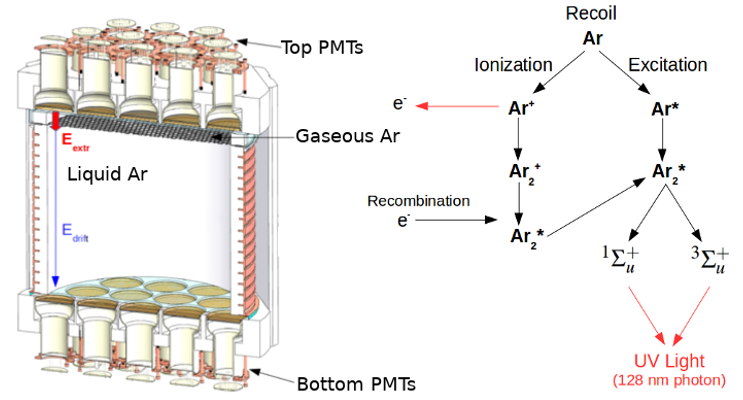
\includegraphics[scale=0.5]{images/detector.png}
\caption{\cite{edkins2017detailed} Schematic of a LAr-TPC and processes of VUV photon emission.}
\label{fig:detector}
\end{figure}
\par Finally, to understand the variables of interest in this study consider Figure \ref{fig:detector}.
A dark matter particle enters the detector fiducial volume where it interacts with an $^{40}\mathrm{\text{Ar}}$ nucleus.
The nucleus then becomes excited and during de-excitation emits electrons and produces scintillation.
This first scintillation is known as $S_1$ and has a windows of 7$\mu$s.
After which the electrons drift upwards due to an electric field, within a window of 376$\mu$s.
The electrons reach a boundary between Argon in the liquid and gaseous phase which produces a secondary, much more intense scintillation.
Subsequently these photons are detected by the Silicon photomultiplier tubes (SiPMTs) and are known as $S_2$; This window of scintillation is about 30$\mu$s.
The ratio of ionization to scintillation is lower for nuclear recoils than for electron recoils and therefore can be used to place selection cuts to increase sensitivity of the detector.
\\
\par There is a further variable used in the discrimination between background (electron recoils) and nuclear recoils.
This is known as the pulse discrimination shape and relates to the de-excitation modes of the Argon nucleus post-recoil.
As illustrated by Figure \ref{fig:detector} there are two excited states $^{1}\mathrm{{\Sigma_{u}}^{+}}$ and $^{3}\mathrm{{\Sigma_{u}}^{+}}$.
The former has a lifetime of 7ns while the latter has a lifetime of 1600ns.
This difference makes Argon a very competitive candidate as a noble element target since this same difference in lifetimes between
excited states in Xenon (the other major competitor for choice of noble element) is only about 25ns.
Although Xenon has other benefits and Argon has other sources of background Xenon based dual phase TPCs do not have, for LAr-TPC based
detectors this feature is a very good discriminant.
This is due to the fact that the ratio of these excited state lifetimes is related to the stopping power or deposited energy per unit path length
$\frac{dE}{dx}$ and this differs between electron recoils such as gamma photons or alpha particles and
nuclear recoils with argon ion tracks.
Thus a parameter is used called the Pulse Shape Discriminant denoted by $f$ subscripted by the window of time of interest in ns.
We shall use $f_{200}$ defined as
\begin{equation}
f_{200}=\frac{\int_{0}^{200ns}\text{Intensity of photons received}}{\int_{0}^{7\mu s}\text{Intensity of photons received}}.
\end{equation}
Illustrated in Figure \ref{fig:psd} is the simulated difference in Darkside-20k between nuclear and electron recoils for $f_{200}$ against total $S_1$ intensity.
Although historically the parameter $f_{90}$ has been used for experiments such as Darkside-50, for a much bigger experiment such as this the drift distance is increased substantially so
$f_{200}$ is more suitable.
\begin{figure}[H]
\begin{minipage}{.49\textwidth}
  \centering
  \begin{subfigure}{\textwidth}
      \centering\captionsetup{width=.9\linewidth}%
      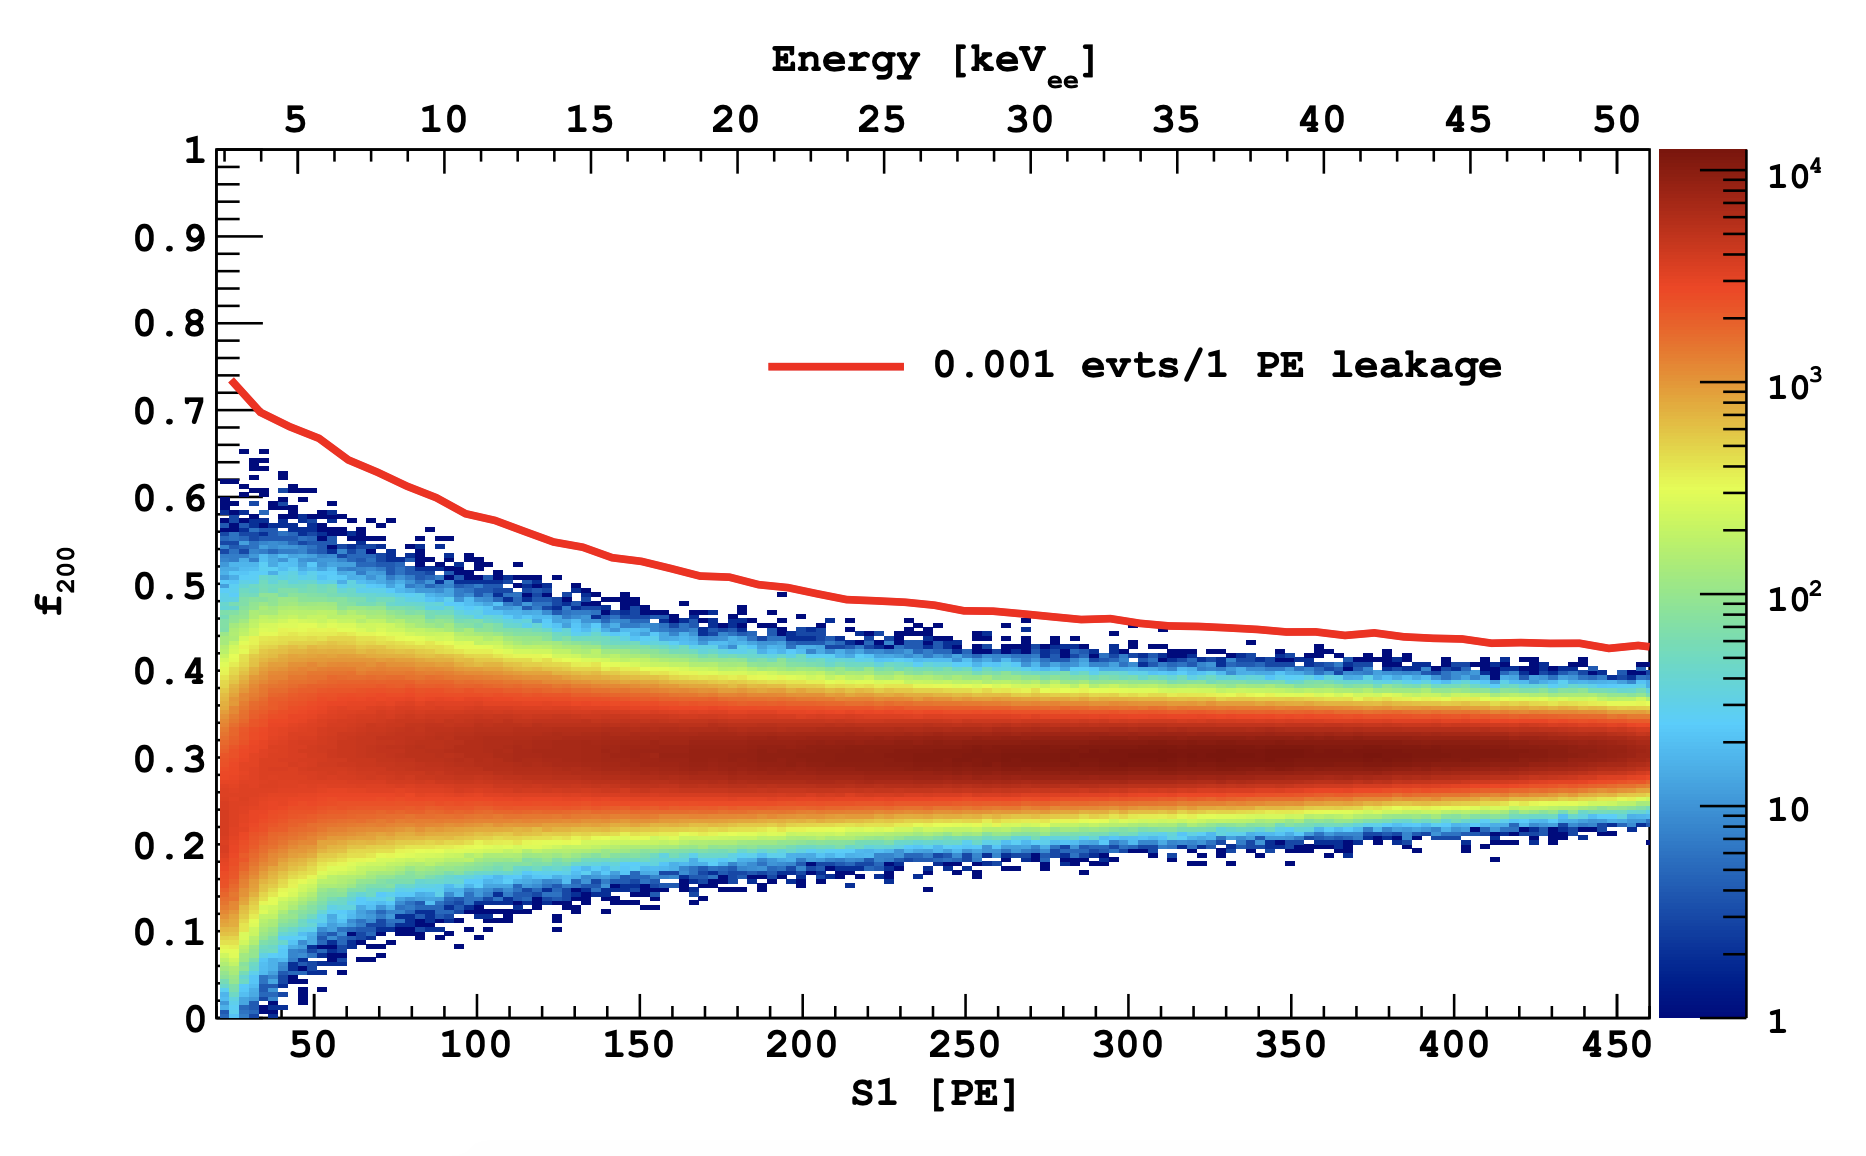
\includegraphics[width=\textwidth]{./images/psd_background.png}
      \caption{Simulations for Darkside-20k of $f_{200}$ vs $S_1$ for background data using $^{39}\mathrm{\text{Ar}}$ $\beta$'s.
      Red line is a leakage curve for a 5-PE requirement on $\beta$'s.}
  \end{subfigure}
\end{minipage}
\begin{minipage}{.49\textwidth}
  \centering
  \begin{subfigure}{\textwidth}
      \centering\captionsetup{width=.9\linewidth}%
      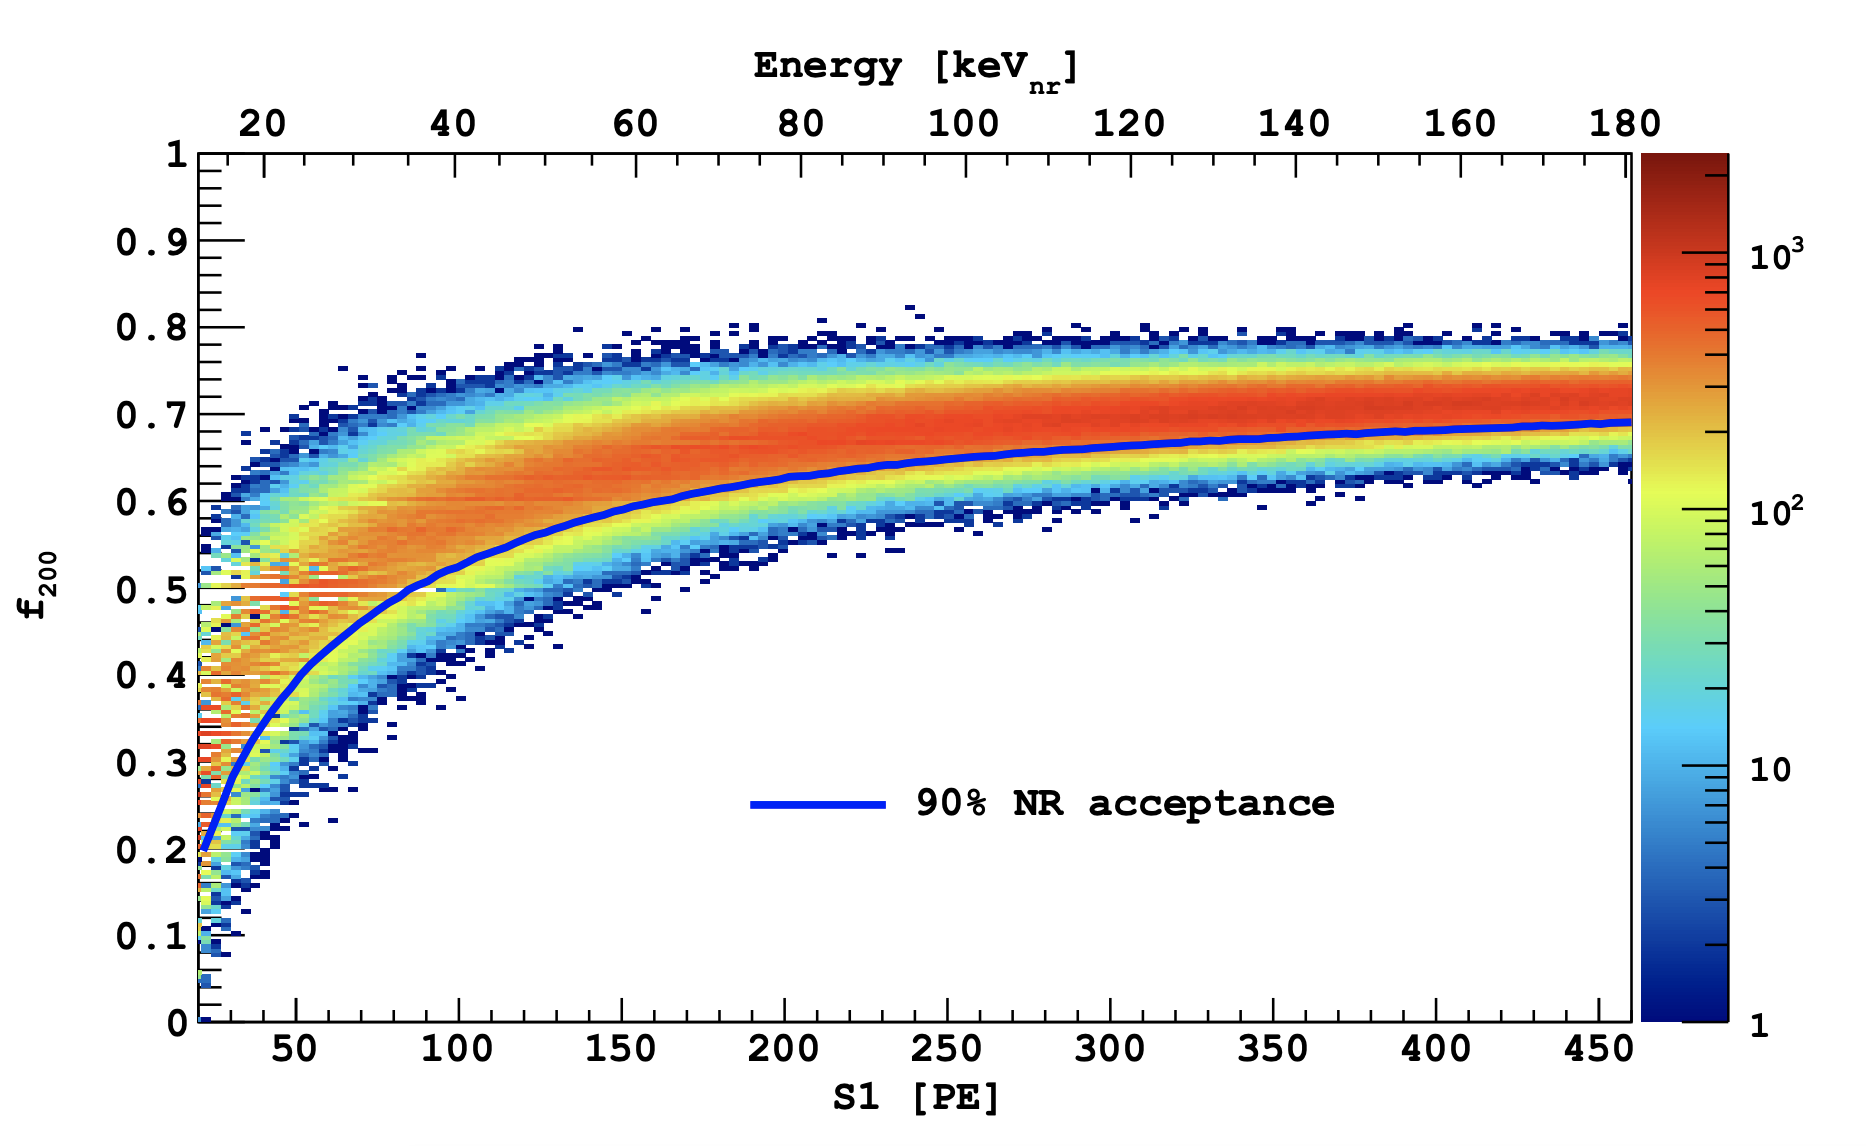
\includegraphics[width=\textwidth]{./images/psd_signal.png}
      \caption{Simulations for Darkside-20k of $f_{200}$ vs $S_1$ for signal nuclear recoils.
      Blue curve is the 90\% NR acceptance region.}
  \end{subfigure}
\end{minipage}
\caption{\cite{aalseth2018darkside} Region of interest using $f_{200}$ pulse shape discriminant against total intensity $S_1$.}
\label{fig:psd}
\end{figure}
\subsection{Current G4DS Results}
The current simulation methods used by the Darkside collaboration consist of very sophisticated and proven Monte Carlo methods.
These have been programmed in an open-source software package called Geant4 \cite{G4} and the complete set of detector macros and routines is called G4DS.
For the purposes of this report and our study we ran G4DS with the following configuration detailed in Table \ref{table:g4ds_config}.
\begin{table}[!h]
\centering
\begin{tabular}{l|l}
\hline
Drift Field & 200V \\
TPC Height & 262cm \\
TPC Width & 150cm \\
Thickness Acrylic Walls & 5cm \\
Thickness LArBuffers & 40cm \\
Thickness Veto Shell & 10cm \\
Thickness TPB & 0.1 mm \\
\hline
\end{tabular}
\caption{Table detailing the major features of the detector setup used in G4DS for the purposes of this study.}
\label{table:g4ds_config}
\end{table}
Although the default configuration was used, no selection cuts were made on any of the data for the purpose of simply studying the reproducing power of the deep learning technique.
We simulated 1000 uniformly distributed events per $^{40}\mathrm{\text{Ar}}$ recoil in the range 5-235 keV in steps of 1 keV.
An example for 1000, 100 keV nuclear recoil events is shown in Figure \ref{fig:example_vars} for each of the three variables $S_1$, $S_2$ and $f_{200}$.
The data for each variable is similar in shape but the ranges are different and the separation in arithmetic means for the 200 different energies is quite small for $f_{200}$
when compared to $S_1$ and $S_2$.
What this means is that there might be difficulty in training a neural network to produce such $f_{200}$ distributions on condition of the energy, since they are not very distinguishable from each other and do overlap.
\begin{figure}[H]
\begin{minipage}{.5\textwidth}
  \centering
  \begin{subfigure}{.9\textwidth}
      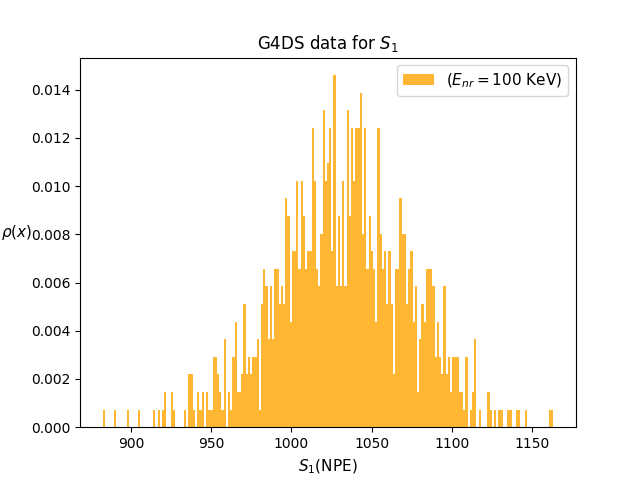
\includegraphics[width=\textwidth]{./images/s1_100.png}
      \subcaption{G4DS generated data for $S_1$}
  \end{subfigure}
\end{minipage}
\begin{minipage}{.5\textwidth}
  \centering
  \begin{subfigure}{.9\textwidth}
      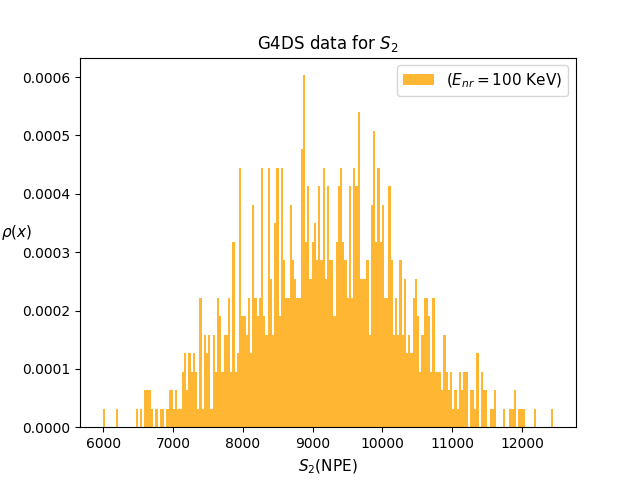
\includegraphics[width=\textwidth]{./images/s2_100.png}
      \subcaption{G4DS generated data for $S_2$}
  \end{subfigure}
\end{minipage}
\end{figure}
\begin{figure}[H]\ContinuedFloat
\centering
\begin{minipage}{.5\textwidth}
  \centering
  \begin{subfigure}{.9\textwidth}
      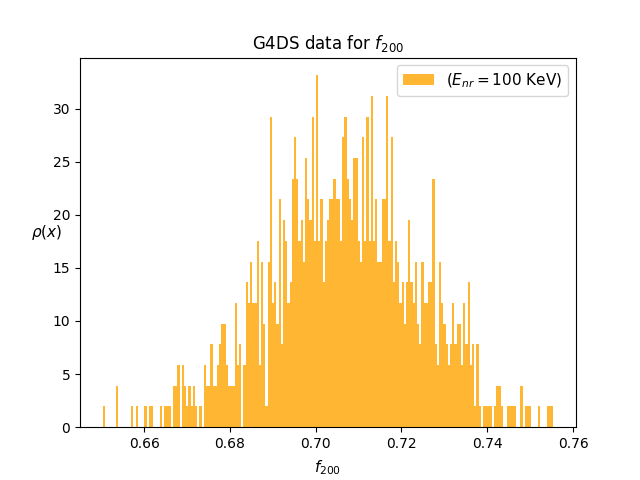
\includegraphics[width=\textwidth]{./images/f200like_100.png}
      \subcaption{G4DS generated data for $f_{200}$}
  \end{subfigure}
\end{minipage}
\caption{Example of the generated data for a run of 1000, 100 keV $^{40}\mathrm{\text{Ar}}$ recoils in G4DS.}
\label{fig:example_vars}
\end{figure}
\par The neural networks described in the next section will therefore be trained on these types of distributions and finally we will want to reproduce
plots such as Figure \ref{fig:psd} to check that the correlation between the three variables has been understood to an acceptable extent.

\subsection{Deep learning as an alternative}
As discussed before, the results obtained with G4DS are well understood and accepted as correct simulations (backed up by experiments DS50 \cite{agnes2015first}).
However, with great detail come large amounts of time waiting for the simulations to complete.
Moreover anytime the nuclear recoil spectrum is changed to simulate different masses of WIMPs, the simulations must be run again.
This hinders progress that can be made to an extent since instead of being able to test multiple theories, one must take great care to compromise with time spent waiting and computational resources needed.
Lastly, a solution to this could be increasing the number of processors, GPUs and computing capabilities but these cost a lot of money and do not necessarily scale linearly.
It would also be improbable for an institution or a department with a fixed budget it must stick to, to assign more and more resources to one research group which means this is
not a sustainable solution.
\\
\par This is where neural networks appear as a possible solution to this problem.
The following is not an introduction to machine learning techniques, rather for that please refer to my first semester report \cite{firstsemester}.
A neural network is a set of nodes in different, successively connected layers.
Each layer contains many nodes connected to other nodes from successive and previous layers.
Each of these nodes carry intermediary weights to certain functions of output.
In a forward run, the input layers (containing the data to be trained) are connected to
intermediary layers whom carry out some transformation or apply a so called 'activation function' to give
the intermediary weights some values.
This is repeated until the final layer is reached which will usually have an activation function which is dependent on the type of problem at hand.
For example, a classification problem will have weights representing each category which will be largest for the category the algorithm classifies the input as and lower or 0 for the others.
These final weights are then compared to what they should be from the known labelled training data and a quantity to measure 'goodness' of the algorithm is set.
The function doing this measure is called the loss function.
Acting on this number will be an optimizer which then changes the intermediary weights accordingly so that ideally on the next run
the new weights and activation functions will guide the algorithm towards better final weights which will minimize loss and maximise accuracy.
\\
\par This is actually only one type of machine learning known as supervised learning.
The other kind, unsupervised learning, is what we carry out in the algorithms detailed in this report where we essentially implement dimensionality reduction.
Particularly, we make use of a rather new method of machine learning known as Generative Adverserial Networks \cite{NIPS2014_5423} \cite{salimans2016improved}.
In our case we have two neural networks, one known as the classifier and the other as the generator.
The aim of the generator is to reproduce training data as close as possible while the job of the classifier is to
spot at each iteration of training (known as an epoch) which of the two inputs it is being presented with, real or generated.
Their loss functions, for a fixed generator G and the optimal discriminator $D^*_G(\bar x)$ is given by minimizing the function \cite{NIPS2014_5423}
\begin{equation}
  C(G)=\E_{x\sim p_{data}}[\log (D^*_G(\bar x)]+\E_{x\sim p_{g}}[\log(1-D^*_G(\bar x)]
  \label{eq:minmax}
\end{equation}
where the optimal discriminator is described by
\begin{equation}
  D^*_G(\bar x)= \frac{p_{data}(\bar x)}{p_{data}(\bar x) + p_{g}(\bar x)}.
  \label{eq:optimal_disc}
\end{equation}
\\
For the ideal case where the generator is perfect the accuracy of the discriminator is expected to be
around 0.5 as it would have no real clue other than a 50-50\% chance to tell the difference between real and generated data.
\section{Methods}
\subsection{Problems with previous approach}
In the first semester, a qualitative approach was taken to this problem of trying to reproduce G4DS data through a GAN.
Moreover, we required a cGAN, or conditional GAN, which would accept as a condition the nuclear recoil energy E and produce the corresponding $S_1$, $S_2$, $f_200$.
The results of that report showed promising reproductions of the real data but there were three main problems with that approach:
\begin{enumerate}[i)]
  \item There was barely any quantitative analysis of the reproducability of training data by the GAN.
  This was done mainly by visually looking at any two same energy plots for a particular variable since the main aim was to check that if such an algorithm would even be possible.
  \item As we trained the GAN to learn $P(S_1|E)$ and then $P(S_1 \cap S_2|E)$ and so on the network created was exponentially larger and more complicated.
  It was not only a matter of adding more layers or nodes but required for each variable a substantial rethinking of the networks (generator and discriminator) as a whole every time.
  \item The 3D, 1 conditional GAN was not able to learn the 3 variables at once and we had to abandon this path quickly since it did not produce any returns on effort put in.
\end{enumerate}
\subsection{Novel techniques}
\subsubsection{Wasserstein GANs}
As a result of this we expanded our search for a different architecture of GANs.
At the end of last semester we identified wGANs, or Wasserstein GANs \cite{arjovsky2017wasserstein}, to be the next architecture we would try.
The main feature of this GAN is that it uses a different loss function, or way of quantifying how bad the generator output is from the real data.
The problem with this is that although initially we thought this difference was only about modifying the loss function and some minor tweaks in the code,
initial results quickly highlighted this was fundamentally a different architecture we were dealing with.
This would have meant spending close to the same amount of time as the first semester, trying to get essentially to the same point we already had got.
This architecture promised better convergence in less epochs and is proven to be much better in terms of performance than the minmax approach taken by the
underlying loss function of the traditional/vanilla GAN but this was not the aim of what were doing.
We thus decided to focus our efforts on other architectures.
Lastly, we are thus not saying wGANs are not worth implementing, rather from what we observed during
proof of concept training they are very efficient but quickly end up in failure modes if not configured well.
So we do suggest this architecture be studied in the future, perhaps in the next iteration of this project since it could potentially
save many epochs worth of work and achieve even better convergence.
\subsubsection{ARGANs}
Even though I admit it is hard to believe, the name has nothing to do with the fact we are using this in a liquid Argon TPC.
In fact, AutoRegressive GANs \cite{yazici2018autoregressive} \cite{zhao2019compression} have been first called so in 2018 but the underlying theory has been used in the context of machine learning for decades now.
Although mostly used in the ambit of image generation the method still applies to our problem.
In reality, the ARGAN proposed in 2018 actually made use of modeling data in the latent (feature) space rather than data space like the older
employers of this method have \cite{fu2019time}.
The closest to what we have done was done in 2011 \cite{oord2016pixel} when a GAN was used by training it in an image generation context.
Each pixel was trained individually with the condition of all its preceding pixels learnt.
Similarly the probability we are trying to teach our generator in this method is given by
\begin{equation}
  p(\bar x)= \prod_{i=1}^np(x_i|x_0,...,x_{i-1})
  \label{eq:prob_dist}
\end{equation}
where in our case $i$ runs from 1 to 3 for $S_1$, $S_2$, $f_200$ and $i=0$ is the recoil energy E.
More explicitly, $P(S_1|E)$ was taught for s epochs (usually 10,000 in this report) and the best output of that generator was
passed to $P(S_2|S_1,E)$ to be trained for a further 10,000 epochs and again to obtain $P(f_{200}|S_2,S_1,E)$.
The massive advantage of this is that essentially we are training 1DcGANs (where the dimension is the number of variables being taught) and
by the end of the process we have trained the three variables with their joint porbabilities, all from a single energy input.
Moreover, the complexity of this architecture is comparable to the 1D vanilla cGAN rather than the 3D cGAN.
Lastly, in my personal opinion as an advocate for scalability and future-proofing, we are making sure that if the collaboration's needs
are ever changed so as to require the need to train a further variable, this can be easily done.
Unless this new variable is wildly different than the three already taught chances are that a very similar neural network can be used.
\subsubsection{Moments as a measure of performance}
One of the conclusions from last semester was the need for more detailed metrics to compare generator and discriminator
performance while training.
We used to monitor performance using the discriminator accuracy/loss vs epoch curve.
Ideally the accuracy would converge to about 0.5 and loss to about 0.7 however beyond checking this convergence
those plots do not convey much information.
In fact, because of an effect GANs are known to enter known as a failure mode (where the generator and the discriminator
reach a Nash equilibrium \cite{salimans2016improved}) the accuracy/loss plot would
show convergence towards expected values but the generated data would be nowhere close to the training data.
One can compare this plot in Figure \ref{fig:acc_loss} with Figure \ref{fig:moments} explained hereunder.
While comparing these plots bear in mind that this run ended up not converging for $f_{200}$ and it is fair to assert that
Figure \ref{fig:moments} does a much better job at showing this than Figure \ref{fig:acc_loss}.
\begin{figure}[H]
\centering
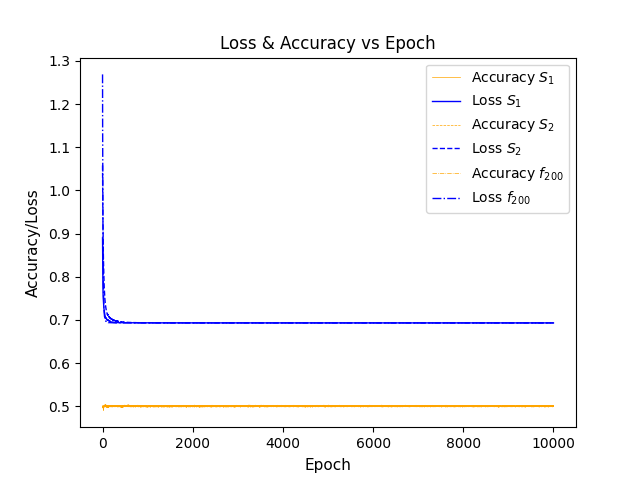
\includegraphics[width=0.65\textwidth]{./images/performance.png}
\caption{Previously used in semester 1, these accuracy/loss curves clearly do not convey enough
information about convergence and performance of the GAN during training.}
\label{fig:acc_loss}
\end{figure}
\par
A new metric would not only allow us to better compare how different GAN configuration affect performance but also
in real-time give us the opportunity to gauge if the current configuration being used is likely to converge.
Of course we are not the first people to have to compare two distributions together.
We needed something fast during training to not hinder the already cumbersome process so, although metrics
such as Wasserstein distance are ideal, we carry out these metrics after training in the analysis stage.
We also needed something that would not necessarily give us granular detail of performance but more
of a global gauge of how the GAN is performing across the whole energy domain, per variable.
\\
\par Thus we settled on selecting three energies from the whole 230 energy samples being trained on simultaneously.
These three energies were specifically selected to be the first, middle and last in the domain.
Then, the array of length 3 arrays of length 1000 data points each is flattened and the first and second moments are calculated.
The ratio of $\frac{\E(\text{GAN4DS Output})}{\E(\text{G4DS Output})}$ and $\frac{\Var(\text{GAN4DS Output})}{\Var(\text{G4DS Output})}$ is obtained.
Figure \ref{fig:moments} shows these ratios plotted at every epoch check (which in this run was at every 100 epochs) for a particular run
which ended up not converging for $f_{200}$.
One thing to note is that we are suggesting these plots alongside the accuracy/loss curves since a convergence in the latter
but non convergence in the former is the best way to observe failure modes, which is an added advantage to having these new plots.
\\
\par Finally, at every epoch check after logging these ratios we also check if this generator is the best one yet.
The way we do this is to calculate Taxicab metric on each energy histogram between GAN4DS and G4DS and sum the distances for all the energies in the domain.
Then we check if this is less than the previous sum of distances and if it is we save this particular run.
This allows us to save the generator that most closely resembles the training dataset, using this metric.
At the same time Tensorflow is trying to minimize the value of the loss.
As a potential extension and given the promising results the ratio plots have shown us, we
suggest using this metric in the future by including it directly into the Tensorflow network layout as a metric alongside loss minimization.
\begin{figure}[H]
\centering
\begin{minipage}{\textwidth}
  \begin{subfigure}{.5\textwidth}
      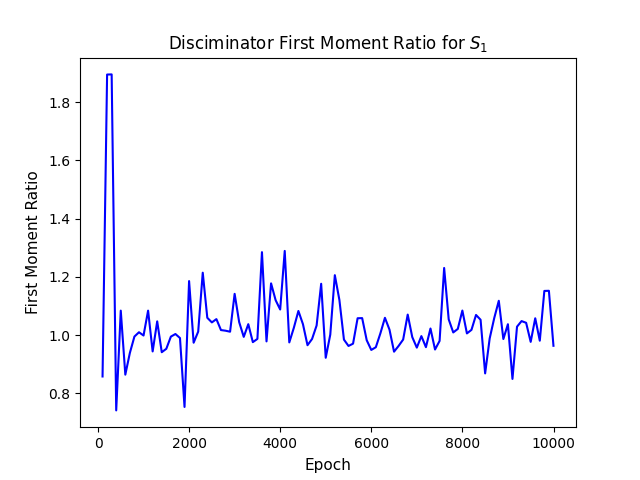
\includegraphics[scale=0.6]{./images/moment_1_s1.png}
      \subcaption{Ratio of first moment for $S_{1}$}
  \end{subfigure}
  \begin{subfigure}{.5\textwidth}
      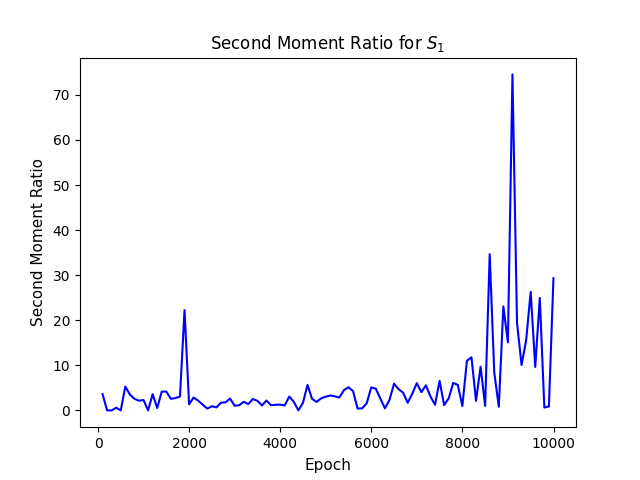
\includegraphics[scale=0.6]{./images/moment_2_s1.png}
      \subcaption{Ratio of second moment for $S_{1}$}
  \end{subfigure}
\end{minipage}
\begin{minipage}{\textwidth}
  \begin{subfigure}{.5\textwidth}
      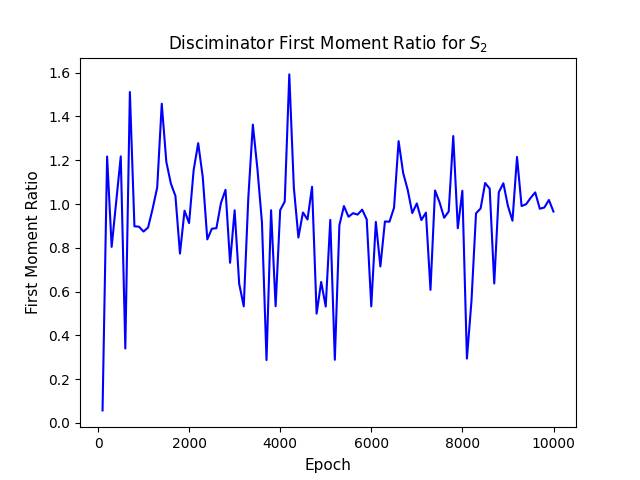
\includegraphics[scale=0.6]{./images/moment_1_s2.png}
      \subcaption{Ratio of first moment for $S_{2}$}
  \end{subfigure}
  \begin{subfigure}{.5\textwidth}
      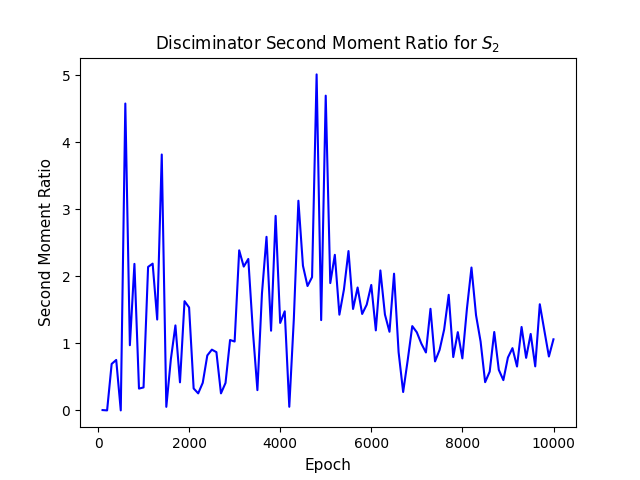
\includegraphics[scale=0.6]{./images/moment_2_s2.png}
      \subcaption{Ratio of second moment for $S_{2}$}
  \end{subfigure}
\end{minipage}
\begin{minipage}{\textwidth}
  \begin{subfigure}{.5\textwidth}
      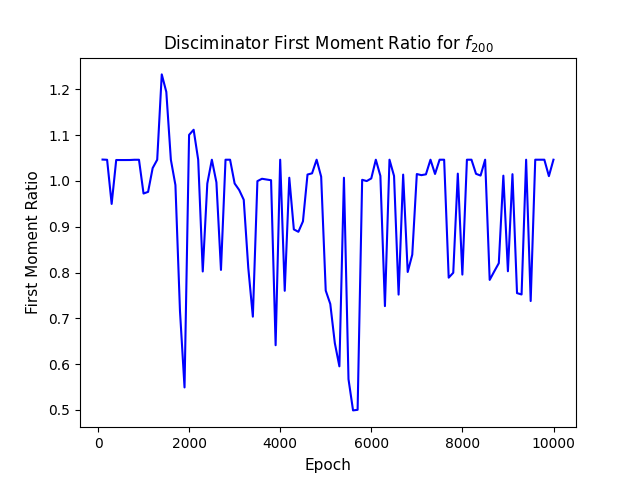
\includegraphics[scale=0.6]{./images/moment_1_f200like.png}
      \subcaption{Ratio of first moment for $f_{200}$}
  \end{subfigure}
  \begin{subfigure}{.5\textwidth}
      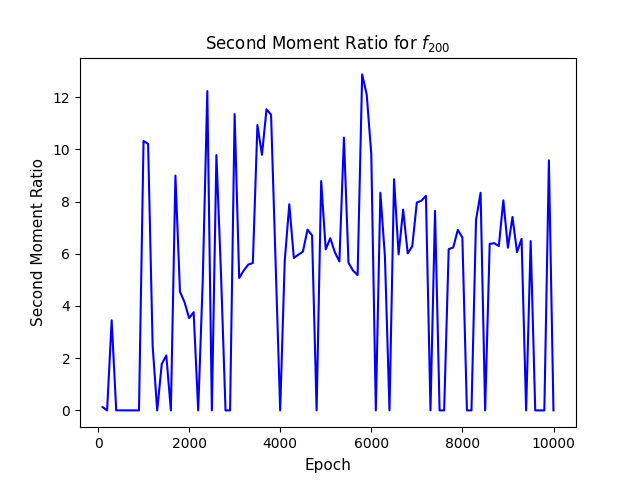
\includegraphics[scale=0.6]{./images/moment_2_f200like.png}
      \subcaption{Ratio of second moment for $f_{200}$}
  \end{subfigure}
\end{minipage}
\caption{Use of ratio of GAN4DS/G4DS moments during training drastically improves the capture of the actual performance of the GAN
compared to accuracy-loss more commonly used in machine learning.}
\label{fig:moments}
\end{figure}
\subsubsection{Work Pipeline}
Before presenting final results, I thought it might be worthwhile briefly mentioning changes to our
coding style and the way we completely redefined our work pipeline.
Last semester we found working on an online, free platform provided by Google called Colab helped us work together thus sharing the same results
and make use of the Python Jupyter notebooks with NVIDIA T4 GPUs which have a 16GB memory needed for the large dataset of training we have.
We found however that we easily ended up with tens of notebooks, each with a different architecture and needing to manually save outputs.
Consistency between different notebooks was lacking at best and the biggest drawback was that the session would timeout after a while so the network could not
be let to train for long periods of time reliably.
\\
\par We therefore took the opportunity to convert all of the code to a single Python project to be run on the University of Manchester's Physics Department GPU cluster.
The package we produced aims to really focus on being able to be used in the future by people that might not be aware of the inner workings of machine learning
and instead changes the focus on what the researcher wants to train and what they would like to see it output.
The program takes in the variables and the training dataset (after self-extracting from ROOT files of $\approx$ 1GB per energy to $\approx$ 20kB)
and a layout specified in a markup language independent from the Python code.
The program then automatically splits up the data in as many batches as needed to serve memory requirements, creates the ARGAN structure, opens a monitorable
Tensorboard session and saves all plots and data logs in a single, consistent format.
Tensorboard is a package provided by Google, the creators of Tensorflow, which allows monitoring machine learning progress to the level
where one can see the weights of each individual layer to monitor how they change with epochs.
We actually made use of this to remove any layers or nodes which were essentially useless or redundant or in certain cases were damaging performance and convergence.
We made this codebase in the hope it could serve as a baseline for future teams potentially working on continuing our work and we encourage to expand its capabilities.
\section{Results}
All results unless specified were obtained by using an ARGAN with 10,000 epochs per variable.
The dataset is comprised of 1000 $^{40}\mathrm{\text{Ar}}$ recoils per nuclear recoil energy in the range [5,235] keV in steps of 1 keV.
The order of variables learnt was $S_1$ then $S_2$ then $f_{200}$.
All results presented are from the same run with the above configuration.
\subsection{Individual Variables}
The first results I present are the individual variables.
Figure \ref{fig:ind_results} shows (left) the results of 3 nuclear recoil energies (minimum, middle and maximum over the recoil energy domain)
of training dataset overlayed with the best GAN output per variable and
(right) the differences for each two equal energy, equal variable counts.
Figure \ref{fig:ind_results_metrics} shows the metrics used to monitor performance during training.
\\
\par The difference plots seem to show a symmetry about the mean of each training dataset distribution.
The GAN appears to have produced output which on one side under-estimates the training data and over-estimates it
on the other side.
The largest difference is seen in the lower energies of the $f_{200}$ distribution.
This could be attributed to the much more spread-out shape these lower energies have when compared to the larger energies.
GANs are known to suffer in datasets where there is high variance across members.
\begin{figure}[H]
\centering
\begin{minipage}{\textwidth}
  \begin{subfigure}{.5\textwidth}
      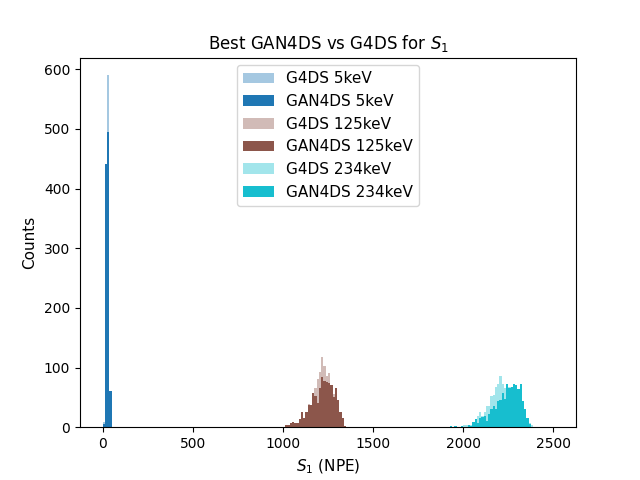
\includegraphics[scale=0.6]{./images/best_s1.png}
      \subcaption{G4DS.}
  \end{subfigure}
  \begin{subfigure}{.5\textwidth}
      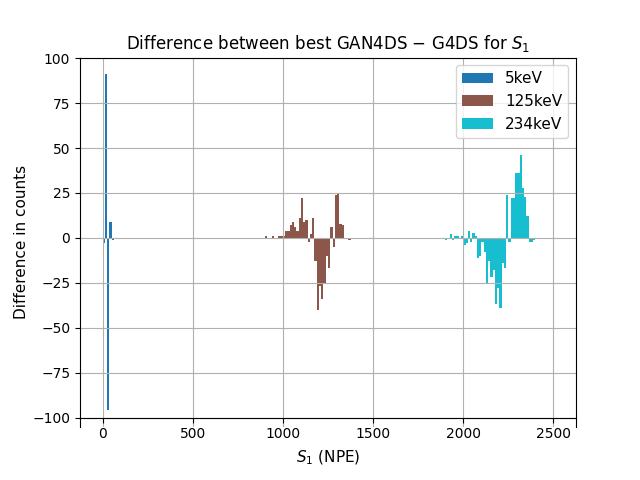
\includegraphics[scale=0.6]{./images/difference_best_s1.png}
      \subcaption{G4DS.}
  \end{subfigure}
\end{minipage}
\begin{minipage}{\textwidth}
  \begin{subfigure}{.5\textwidth}
      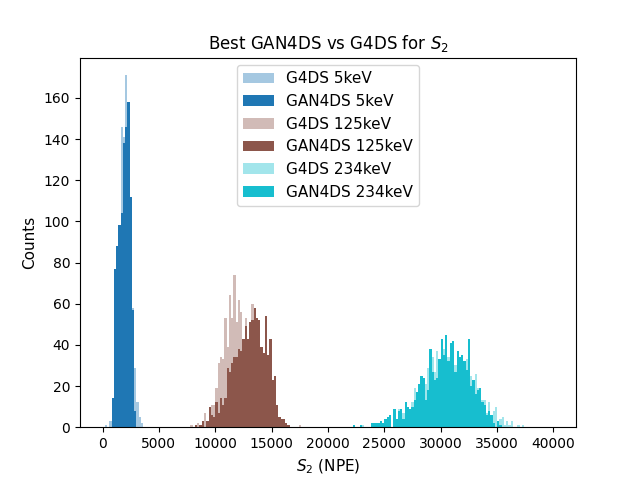
\includegraphics[scale=0.6]{./images/best_s2.png}
      \subcaption{G4DS.}
  \end{subfigure}
  \begin{subfigure}{.5\textwidth}
      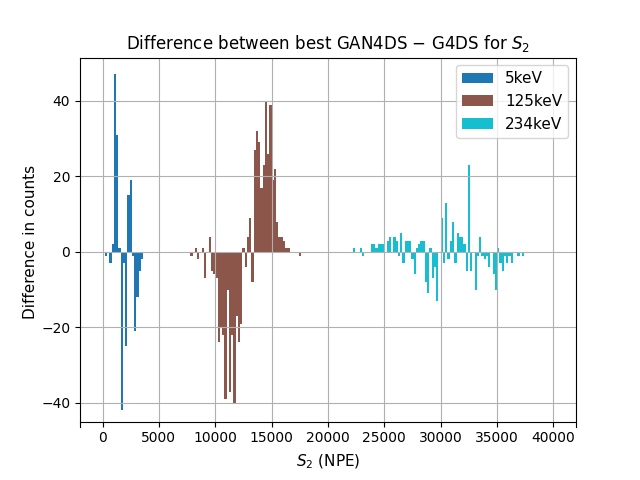
\includegraphics[scale=0.6]{./images/difference_best_s2.png}
      \subcaption{G4DS .}
  \end{subfigure}
\end{minipage}
\begin{minipage}{\textwidth}
  \begin{subfigure}{.5\textwidth}
      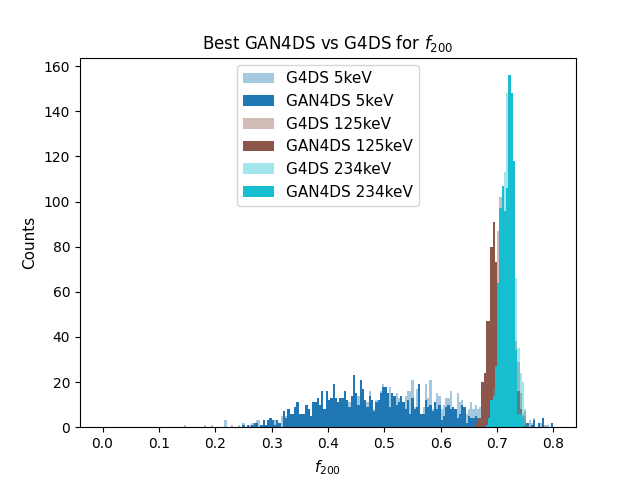
\includegraphics[scale=0.6]{./images/best_f200like.png}
      \subcaption{G4DS.}
  \end{subfigure}
  \begin{subfigure}{.5\textwidth}
      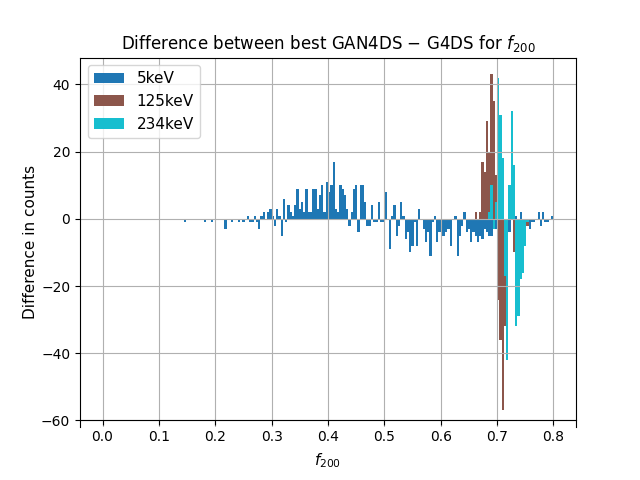
\includegraphics[scale=0.6]{./images/difference_best_f200like.png}
      \subcaption{G4DS.}
  \end{subfigure}
\end{minipage}
\caption{Individual variables learnt successively with each variable adding itself as an input condition
to the next variable being trained. Direct comparisons between generated and trained data to the left, differences per bin on the right.}
\label{fig:ind_results}
\end{figure}
\newpage
\null
\vfill
\begin{figure}[H]
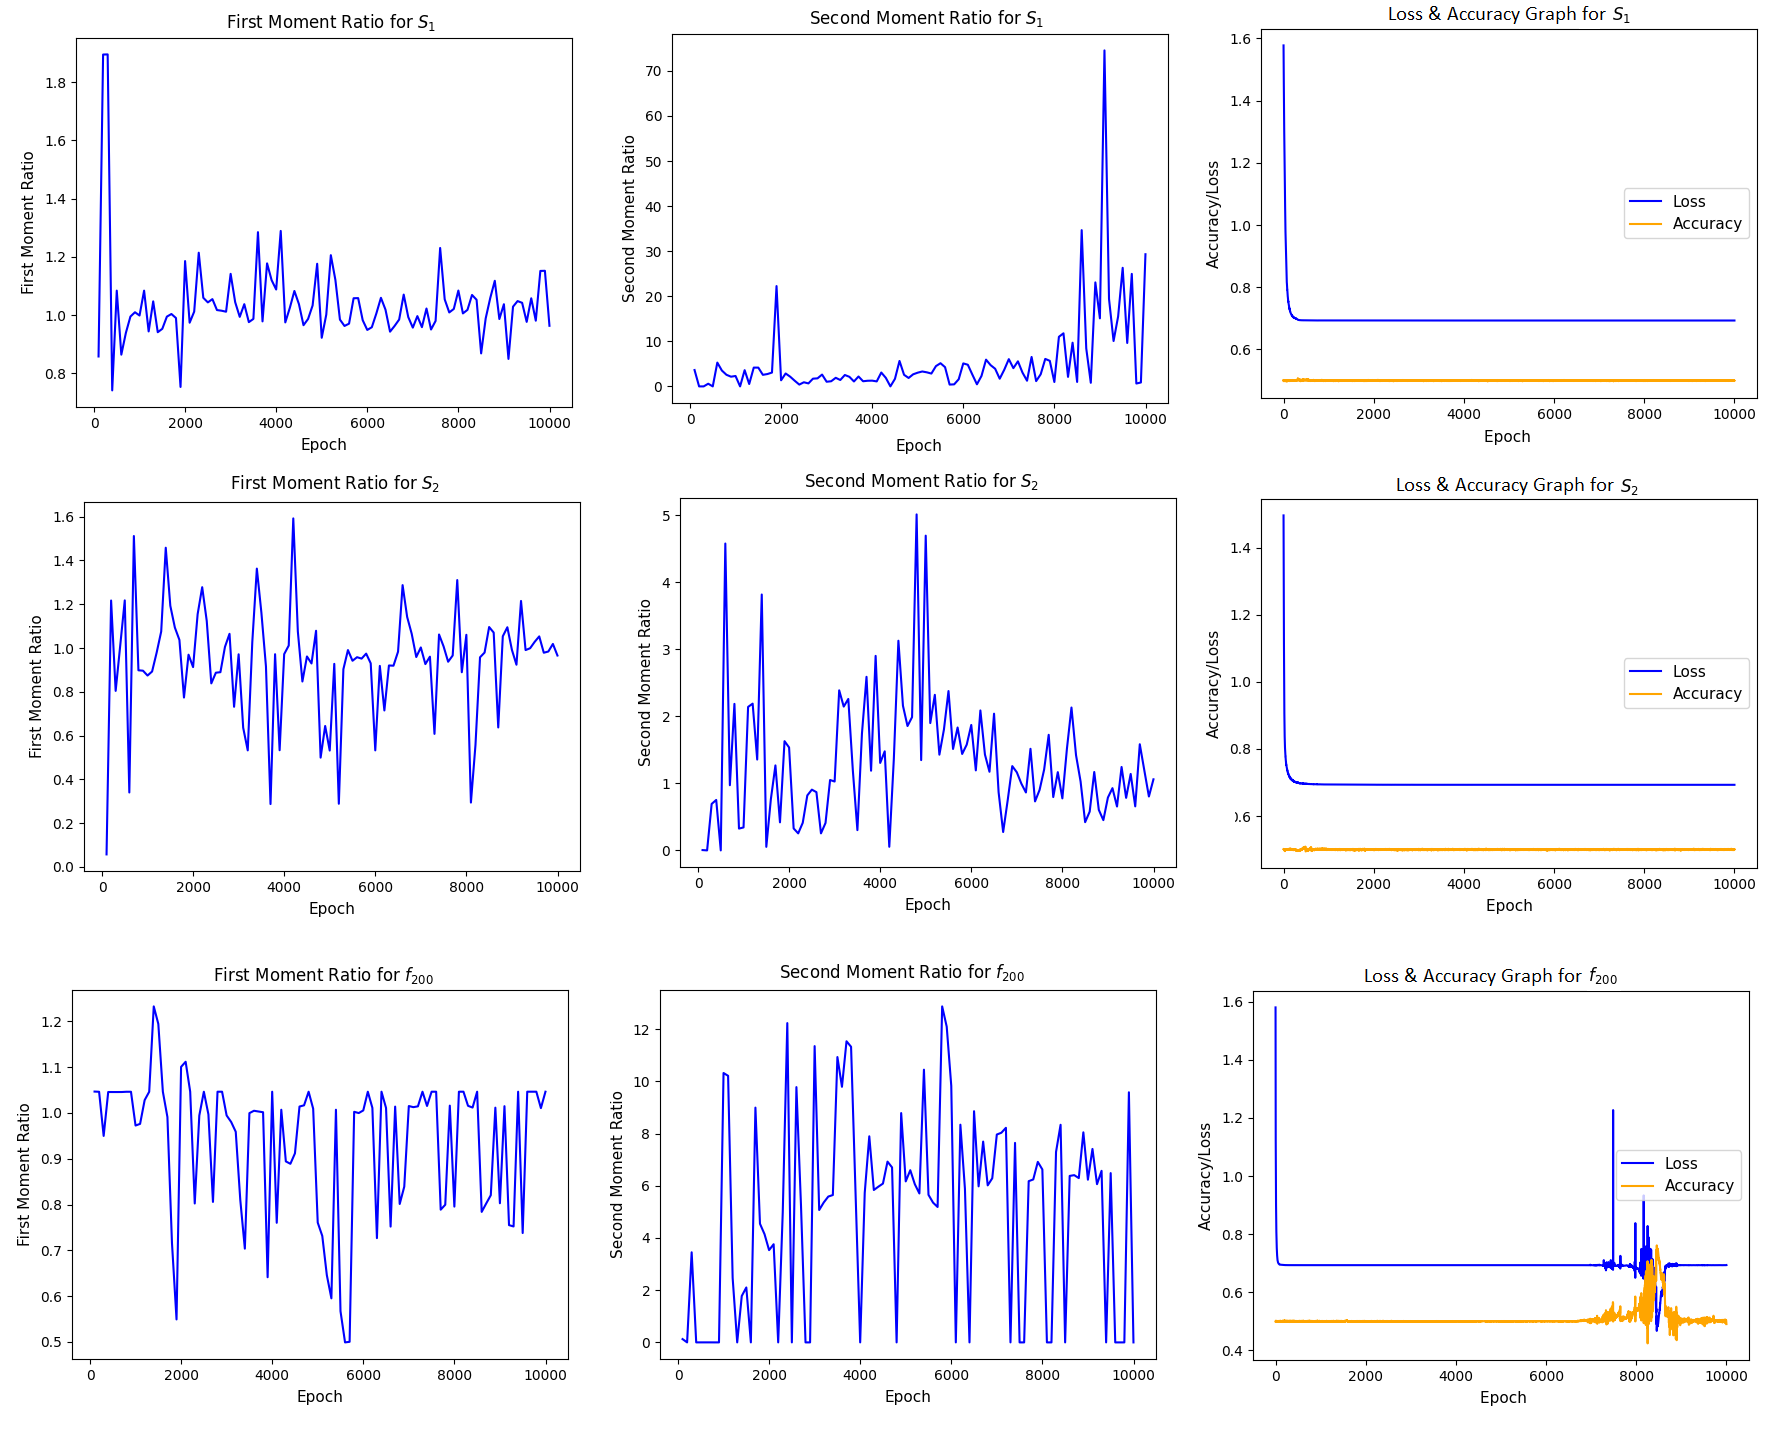
\includegraphics[scale=0.47]{./images/working_metrics.png}
\caption{The metrics used during training to capture performance and convergence
of the GAN on training data.
 From the accuracy/loss plot and the moments plots it appears the GAN had entered a failure mode for $f_{200}$ but
 comes out of it to converge on the actual training data at around 8000 epochs.}
\label{fig:ind_results_metrics}
\end{figure}
\null
\vfill
\newpage
\subsection{Variable Correlations}
Although individual variables are very important, what we sought out to teach the GAN were the correlations between these.
Figures \ref{fig:corr_results_1_5} (log$(m)=1.5$) and \ref{fig:corr_results_4} (log$(m)=4$) show the results for correlations between
the individual variables shown previously.
To produce these correlation plots first a mass for the WIMP is chosen, in this case we take log$(m)=1.5$ and log$(m)=4$ in a spin-independent model which corresponds to a 31.5 GeV/$c^2$ mass.
From theory the corresponding recoil energy spectrum is chosen, shown by Figure \ref{fig:recoil} for log$(m)=$1.5.
After sampling 1000 energies these are used to select from runs of 1000 $^{40}\mathrm{\text{Ar}}$ recoils in G4DS and GAN4DS.
\begin{figure}[H]
\centering
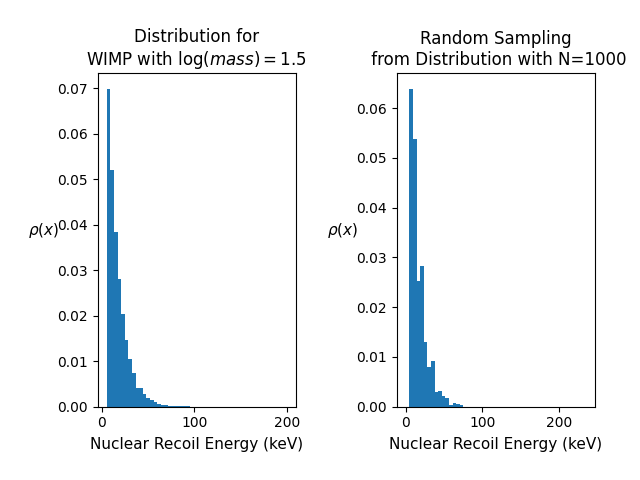
\includegraphics[scale=0.6]{images/Ar_c1dat_m1-5.png}
\caption{A plot of the theoretical recoil energy spectrum for a WIMP of mass log$(m)=1.5$ vs the
sampled N=1000 energies spectrum. The same is done for log$(m)=4$.}
\label{fig:recoil}
\end{figure}
Visually the GAN4DS resembles G4DS very closely both in shape and density.
The band in the $f_{200}$ vs $S_1$ plot in the region of higher energies around the value of $f_{200}\approx 0.7$ is an indication that the correlation was
learnt as this is where signal is expected to lie.
In both \ref{fig:corr_results_1_5}c and \ref{fig:corr_results_1_5}d we see GAN4DS fails to reproduce the low counts of the
outlying points with high variance.
This could be attributed as before to one of the known failures of GANs to reproduce high variance points in training datasets.
One further contribution was the fact that before training, all of the training distributions were normalised
by taking the maximum value for that energy for that variable and dividing by it throughout.
This allowed the GAN to learn how to draw these distributions which were all similar in shape without
being tied to specific magnitudes of mean.
We found that without this normalization before training the GAN mostly fails to learn all the variables.
So although this method we used is very helpful in learning, it might 'squash' the data into the shapes we see and prevent certain points
which have higher variance to be learnt.
\\
\par Finally, the difference plots are very important since they tell us is visually hard to tell.
Again as for the individual variables we notice a kind of symmetry.
This time it is difficult to say why it is symmetric about a certain curve but we hypothesise
this is due to the behaviour also seen in the individual variables.
That is, during training it was observed that the GAN when trying to learn across all the distributions along the energy domain
for a single variable, will try to shift all the distributions together by a fixed amount rather than individually moving
distributions or transforming them.
This was very interesting to see since it could explain a general shift of all the energy distributions as a whole.
Further studies of this might indicate an offset that one could apply to the generated dataset after training
 or a way to penalise the GAN during training when it does this global shifting.
One thing to note is that the difference seems to be less for the higher mass plots and since these have a higher sampling of
higher recoil energy events (conversely a lower sampling of lower energies) it could mean the problem lies in learning the lower energy distributions for each variable.
This is seen later in the analysis subsection.
\begin{figure}[H]
\centering
\begin{minipage}{\textwidth}
  \begin{subfigure}{.5\textwidth}
      \centering\captionsetup{width=.9\linewidth}%
      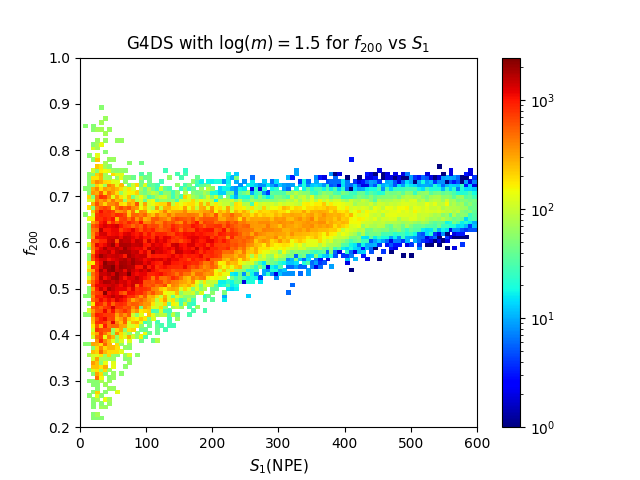
\includegraphics[scale=0.6]{./images/1.5/g4_f200_vs_s1.png}
      \caption{G4DS generated plot for $f_{200}$ vs $S_1$.}
  \end{subfigure}
  \begin{subfigure}{.5\textwidth}
      \centering\captionsetup{width=.9\linewidth}%
      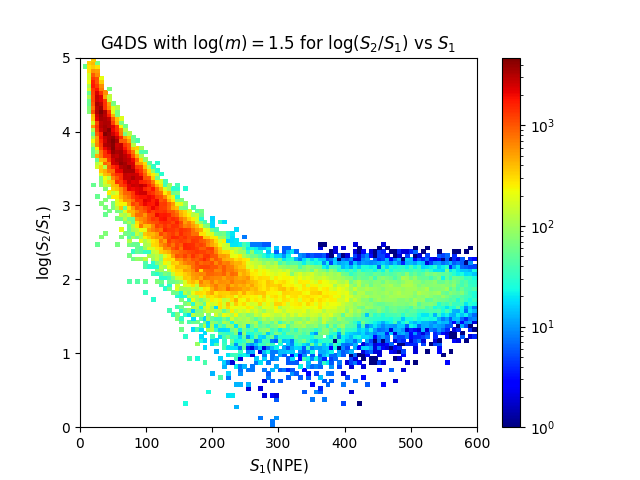
\includegraphics[scale=0.6]{./images/1.5/g4_s1_over_s2_vs_s1.png}
      \caption{G4DS generated plot for log($S_2$/$S_1$) vs $S_1$.}
  \end{subfigure}
\end{minipage}
\begin{minipage}{\textwidth}
  \begin{subfigure}{.5\textwidth}
      \centering\captionsetup{width=.9\linewidth}%
      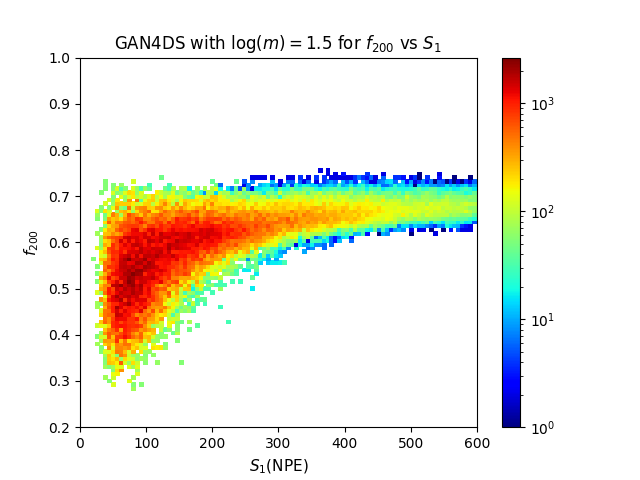
\includegraphics[scale=0.6]{./images/1.5/gan_f200_vs_s1.png}
      \caption{GAN4DS generated plot for $f_{200}$ vs $S_1$.}
  \end{subfigure}
  \begin{subfigure}{.5\textwidth}
      \centering\captionsetup{width=.9\linewidth}%
      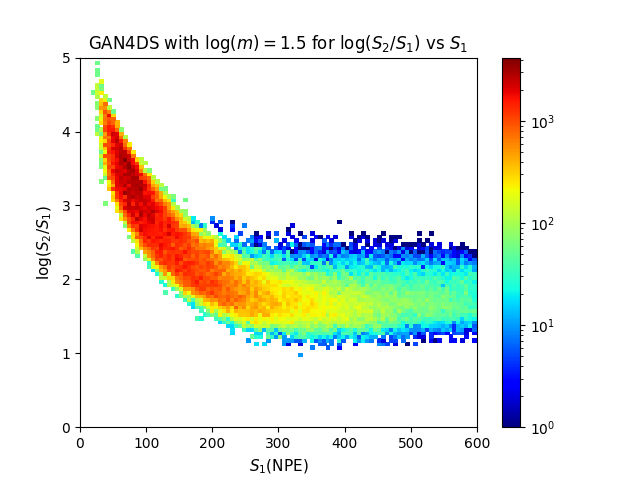
\includegraphics[scale=0.6]{./images/1.5/gan_s1_over_s2_vs_s1.png}
      \caption{GAN4DS generated plot for log($S_2$/$S_1$) vs $S_1$}
  \end{subfigure}
\end{minipage}
\begin{minipage}{\textwidth}
  \begin{subfigure}{.5\textwidth}
      \centering\captionsetup{width=.9\linewidth}%
      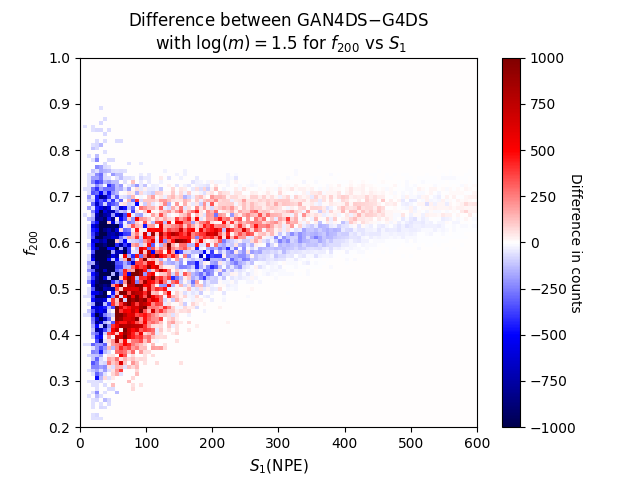
\includegraphics[scale=0.6]{./images/1.5/difference_f200_vs_s1.png}
      \caption{Difference per bin between GAN4DS $-$ G4DS generated data.}
  \end{subfigure}
  \begin{subfigure}{.5\textwidth}
      \centering\captionsetup{width=.9\linewidth}%
      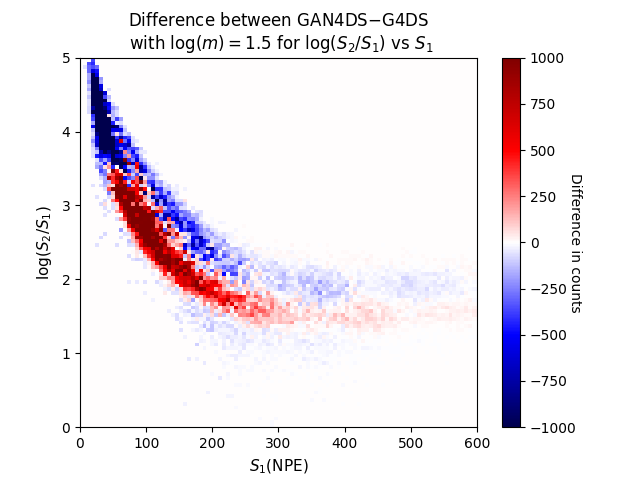
\includegraphics[scale=0.6]{./images/1.5/difference_s1_over_s2_vs_s1.png}
      \caption{Difference per bin between GAN4DS $-$ G4DS generated data.}
  \end{subfigure}
\end{minipage}
\caption{Results showing correlation learnt between the different variables by GAN4DS for log$(m)=1.5$.}
\label{fig:corr_results_1_5}
\end{figure}

\begin{figure}[H]
\centering
\begin{minipage}{\textwidth}
  \begin{subfigure}{.5\textwidth}
      \centering\captionsetup{width=.9\linewidth}%
      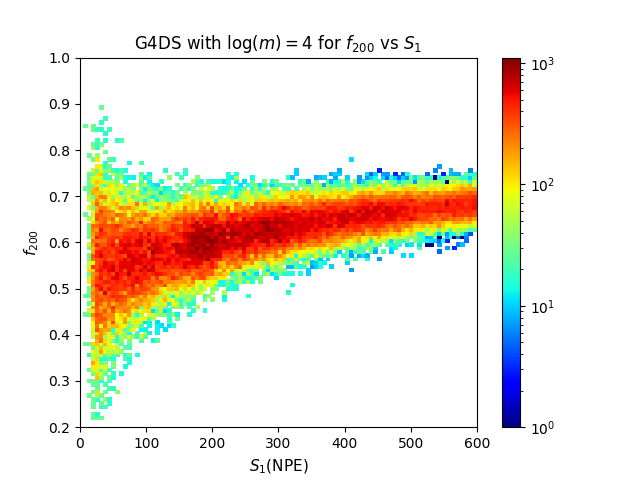
\includegraphics[scale=0.6]{./images/4/g4_f200_vs_s1.png}
      \caption{G4DS generated plot for $f_{200}$ vs $S_1$.}
  \end{subfigure}
  \begin{subfigure}{.5\textwidth}
      \centering\captionsetup{width=.9\linewidth}%
      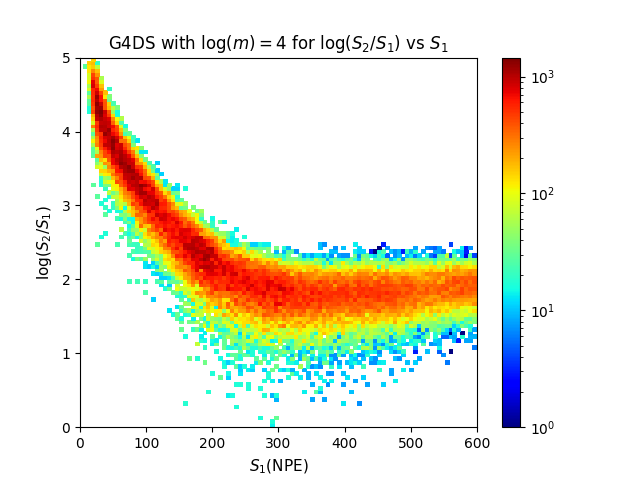
\includegraphics[scale=0.6]{./images/4/g4_s1_over_s2_vs_s1.png}
      \caption{G4DS generated plot for log($S_2$/$S_1$) vs $S_1$.}
  \end{subfigure}
\end{minipage}
\begin{minipage}{\textwidth}
  \begin{subfigure}{.5\textwidth}
      \centering\captionsetup{width=.9\linewidth}%
      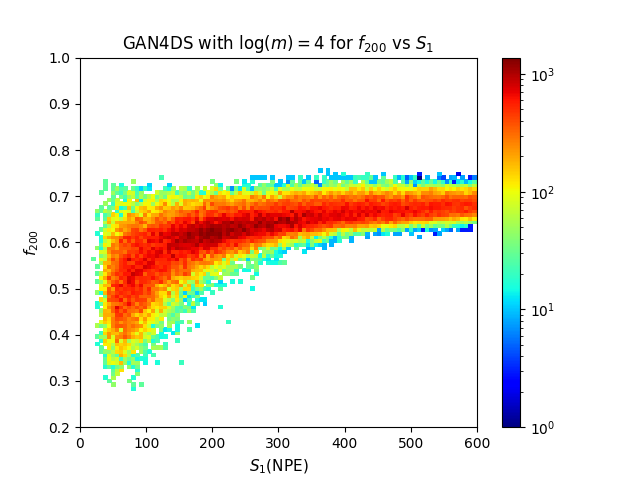
\includegraphics[scale=0.6]{./images/4/gan_f200_vs_s1.png}
      \caption{GAN4DS generated plot for $f_{200}$ vs $S_1$.}
  \end{subfigure}
  \begin{subfigure}{.5\textwidth}
      \centering\captionsetup{width=.9\linewidth}%
      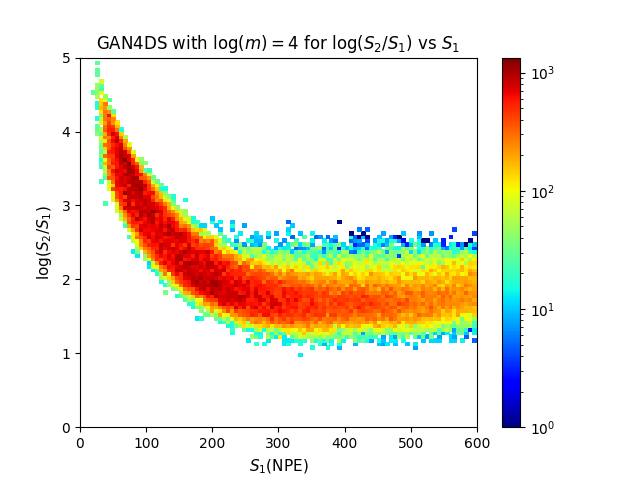
\includegraphics[scale=0.6]{./images/4/gan_s1_over_s2_vs_s1.png}
      \caption{GAN4DS generated plot for log($S_2$/$S_1$) vs $S_1$}
  \end{subfigure}
\end{minipage}
\begin{minipage}{\textwidth}
  \begin{subfigure}{.5\textwidth}
      \centering\captionsetup{width=.9\linewidth}%
      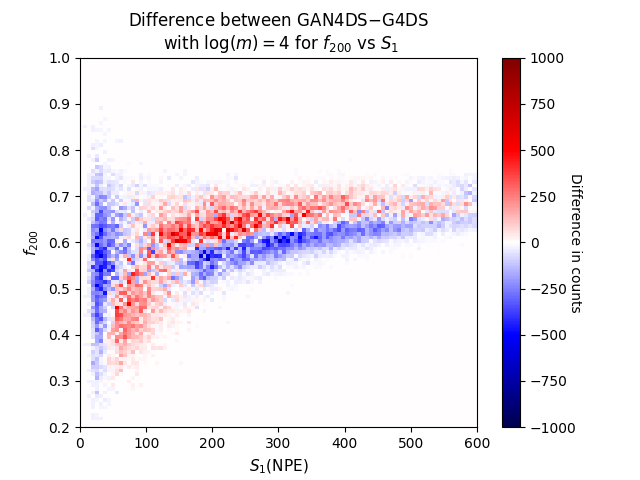
\includegraphics[scale=0.6]{./images/4/difference_f200_vs_s1.png}
      \caption{Difference per bin between GAN4DS $-$ G4DS generated data.}
  \end{subfigure}
  \begin{subfigure}{.5\textwidth}
      \centering\captionsetup{width=.9\linewidth}%
      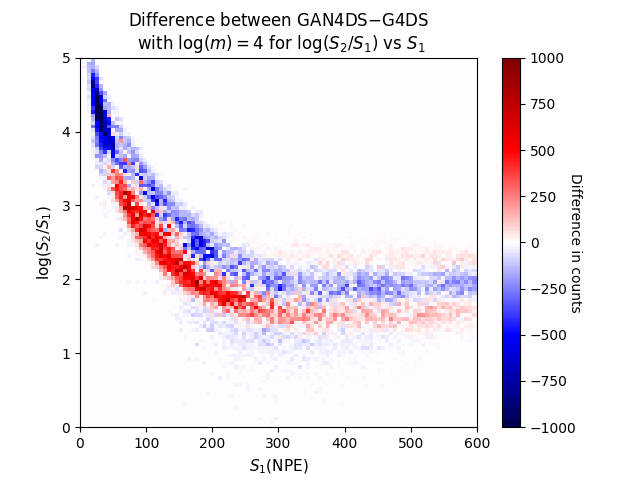
\includegraphics[scale=0.6]{./images/4/difference_s1_over_s2_vs_s1.png}
      \caption{Difference per bin between GAN4DS $-$ G4DS generated data.}
  \end{subfigure}
\end{minipage}
\caption{Results showing correlation learnt between the different variables by GAN4DS for log$(m)=4$.}
\label{fig:corr_results_4}
\end{figure}

\subsection{Accuracy Analysis}
\begin{figure}[H]
\centering
\begin{minipage}{\textwidth}
  \begin{subfigure}{.5\textwidth}
      \centering\captionsetup{width=.8\linewidth}%
      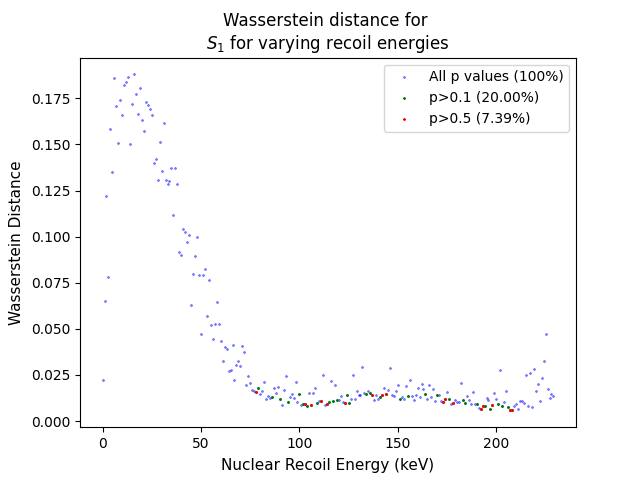
\includegraphics[scale=0.6]{./images/wasserstein_distance_s1.png}
      \caption{G4DS.}
  \end{subfigure}
  \begin{subfigure}{.5\textwidth}
      \centering\captionsetup{width=.8\linewidth}%
      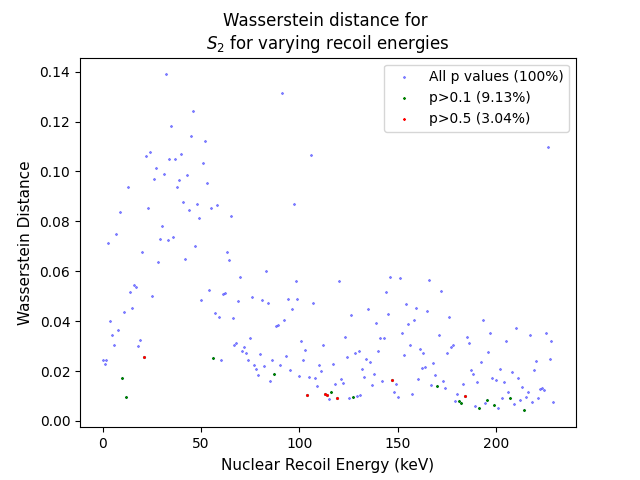
\includegraphics[scale=0.6]{./images/wasserstein_distance_s2.png}
      \caption{G4DS.}
  \end{subfigure}
\end{minipage}
\begin{minipage}{\textwidth}
  \centering
  \begin{subfigure}{.5\textwidth}
      \centering\captionsetup{width=.8\linewidth}%
      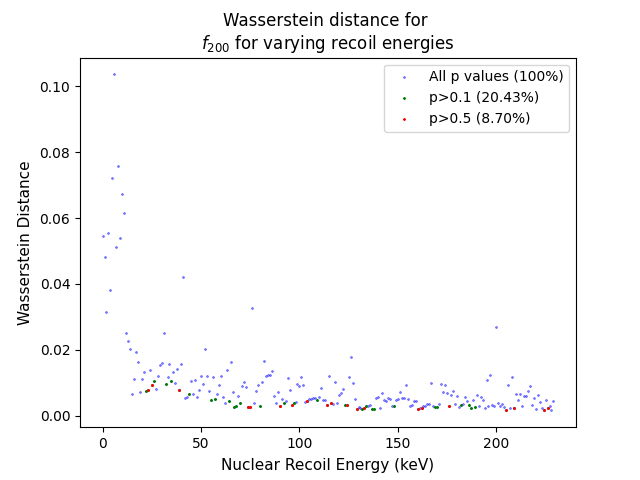
\includegraphics[scale=0.6]{./images/wasserstein_distance_f200like.png}
      \caption{G4DS.}
  \end{subfigure}
\end{minipage}
\caption{Wasserstein metric calculated on the GAN4DS and G4DS generated data for each variable for each energy. P values are
obtained by using a permutation test on geometric mean. In round brackets is the percentage of points that pass the significance threshold.}
\label{fig:wass_distance}
\end{figure}

Figure \ref{fig:wass_distance} shows the results of applying the Wasserstein metric \cite{ramdas2017wasserstein} on each variable for each nuclear recoil energy
between GAN4DS and G4DS.
The Wasserstein metric is often used to compare two distributions together and works on the amount of work/area needed to move around one distribution
to make it equal to the other.
The colours on the points of these plots are due to another test we carried out.
Known as a permutation test \cite{pitman1937significance} \cite{efron1994introduction}, we calculate the geometric mean of the each two equal energy, equal variable distributions and take the absolute difference.
We then mix all the data points from the two and take split them into two groups of random permutations of all the data points.
We then carry out again the difference in geometric mean of the two groups and check if this is at least as extreme as the original geometric mean difference.
This is carried out for 1000 permutations and finally we end up with a probability that if we were to observe another value (have another generated distribution by GAN4DS)
this would have a geometric mean difference with the real data at least as extreme.
Given the Null hypothesis being true, in our case that the two distributions are the same distribution,
this value of p that the permutation test returns will be the confidence we have that we cannot reject the Null hypothesis.
We can never accept the Null hypothesis with this test but only reject it or fail to reject it.
\\
\par The first observation out of these plots is that the GAN reproduces training data much better at higher recoil energies
than lower ones.
This is seen both in the lower Wasserstein distance and the higher amount of points that pass
the permutation test's p significance value.
The even more interesting observation is that the relative distance between variables in the lower energy region
decreases from $S_1$ to $f_{200}$.
Recall these variables were learnt successively and this behaviour seems to show a self-correcting learning behaviour
across variables, not only across epochs.
The pronounced spike in Wasserstein distance between G4DS and GAN4DS for lower recoil energies in $S_1$, seems to disperse for $S_2$ and
for $f_{200}$ again becomes smaller in magnitude and shape.
Essentially, if the GAN does not quite learn how to make this Gaussian-like shaped data for $S_1$, the mistake
is not repeated as a whole for $S_2$ even though the neural network layout used for these two is the same.
Rather, it is appears the more variables trained on the more we can actually see the GAN
getting better at producing these Gaussian-like shapes.
There is one caveat in that Wasserstein distances, as mentioned before, rely on areas so across different variables might not be exactly comparable
however we do normalise each distribution before calculating the Wasserstein distance.
This is done by dividing both GAN4DS and G4DS variable distributions by the same normalisation value as described previously in Section 3.2.
Using this normalization makes the three plots in Figure \ref{fig:wass_distance} more comparable.
\\
\par One final thought is that these results suggest one could benefit in splitting the data around the 75 keV mark into two groups and actually
have a GAN for lower energies and one for higher ones since they are more comparable to each other.
This result also made us question what would happen if one were to insert $S_1$ again after $f_{200}$ has been learnt.
If the Gaussian-like distribution generation has been perfected with each variable, this would make $S_1$ even better than it was originally the first
time it was learnt.
This could potentially be extended to a completely different way of learning.
Instead of learning all the energies for one variable, one could shuffle the variables while keeping the number of energies the same and train over 10,000 epochs.
We suggest this could be one way of doing this, alternatively going through cycles of $S_1$, $S_2$ and $f_{200}$ until the distributions are
learnt for all three variables.
The only way to know whether these approaches or any other ones would work would be to study them
so we hope in future iterations of this project this could be done.
\section{Final Remarks}
Last semester was focused on getting a proof-of-concept GAN working to learn $S_1$, $S_2$ and $f_{200}$ and we managed to show this could be done but not efficiently.
What we have done this semester is make these algorithms scalable and stable and analysed not only qualitatively but quantitively performance and accuracy.
We have tried multiple architectures and finally have settled on the very new ARGANs however this is by no means
the only way to do it nor the best and we definitely encourage new architectures to be tried since this field of research is currently extremely active.
More work has to be carried out in the homogenous learning across all the nuclear recoil energy domain, especially for lower energies.
We suggest doing this by cycling through the variables being taught multiple times in a successive order since we hypothesise this could
really help the GAN converge over the whole energy domain.
\\
\par Finally future extensions to this project could include noise simulations and background simulations and finally all these events put together in one GAN.
An even larger extension would be to generate the individual photon responses by the sensors and PMTs which could then in turn produce the variables studied in this report.
This could potentially be used at the same time to produce directionality predictions by making use of a classifier connected to the output of the GAN.
This would be a massive help to the current detector setup since as of today the detector does not produce such kind of information.
To conclude, we believe this project has produced tantalising results and hope this work will be continued by future iterations of the project.
\newpage
\printbibliography

\end{document}
